% Options for packages loaded elsewhere
\PassOptionsToPackage{unicode,linktoc=all}{hyperref}
\PassOptionsToPackage{hyphens}{url}
\PassOptionsToPackage{dvipsnames,svgnames,x11names}{xcolor}
%
\documentclass[
  11pt,
  a4paperpaper,
  openany,headsepline=on,footsepline=off,DIV=12,table]{scrbook}

\usepackage{amsmath,amssymb}
\usepackage{iftex}
\ifPDFTeX
  \usepackage[T1]{fontenc}
  \usepackage[utf8]{inputenc}
  \usepackage{textcomp} % provide euro and other symbols
\else % if luatex or xetex
  \usepackage{unicode-math}
  \defaultfontfeatures{Scale=MatchLowercase}
  \defaultfontfeatures[\rmfamily]{Ligatures=TeX,Scale=1}
\fi
\usepackage{lmodern}
\ifPDFTeX\else  
    % xetex/luatex font selection
    \setmainfont[]{Roboto}
\fi
% Use upquote if available, for straight quotes in verbatim environments
\IfFileExists{upquote.sty}{\usepackage{upquote}}{}
\IfFileExists{microtype.sty}{% use microtype if available
  \usepackage[]{microtype}
  \UseMicrotypeSet[protrusion]{basicmath} % disable protrusion for tt fonts
}{}
\makeatletter
\@ifundefined{KOMAClassName}{% if non-KOMA class
  \IfFileExists{parskip.sty}{%
    \usepackage{parskip}
  }{% else
    \setlength{\parindent}{0pt}
    \setlength{\parskip}{6pt plus 2pt minus 1pt}}
}{% if KOMA class
  \KOMAoptions{parskip=half}}
\makeatother
\usepackage{xcolor}
\setlength{\emergencystretch}{3em} % prevent overfull lines
\setcounter{secnumdepth}{5}
% Make \paragraph and \subparagraph free-standing
\makeatletter
\ifx\paragraph\undefined\else
  \let\oldparagraph\paragraph
  \renewcommand{\paragraph}{
    \@ifstar
      \xxxParagraphStar
      \xxxParagraphNoStar
  }
  \newcommand{\xxxParagraphStar}[1]{\oldparagraph*{#1}\mbox{}}
  \newcommand{\xxxParagraphNoStar}[1]{\oldparagraph{#1}\mbox{}}
\fi
\ifx\subparagraph\undefined\else
  \let\oldsubparagraph\subparagraph
  \renewcommand{\subparagraph}{
    \@ifstar
      \xxxSubParagraphStar
      \xxxSubParagraphNoStar
  }
  \newcommand{\xxxSubParagraphStar}[1]{\oldsubparagraph*{#1}\mbox{}}
  \newcommand{\xxxSubParagraphNoStar}[1]{\oldsubparagraph{#1}\mbox{}}
\fi
\makeatother


\providecommand{\tightlist}{%
  \setlength{\itemsep}{0pt}\setlength{\parskip}{0pt}}\usepackage{longtable,booktabs,array}
\usepackage{calc} % for calculating minipage widths
% Correct order of tables after \paragraph or \subparagraph
\usepackage{etoolbox}
\makeatletter
\patchcmd\longtable{\par}{\if@noskipsec\mbox{}\fi\par}{}{}
\makeatother
% Allow footnotes in longtable head/foot
\IfFileExists{footnotehyper.sty}{\usepackage{footnotehyper}}{\usepackage{footnote}}
\makesavenoteenv{longtable}
\usepackage{graphicx}
\makeatletter
\newsavebox\pandoc@box
\newcommand*\pandocbounded[1]{% scales image to fit in text height/width
  \sbox\pandoc@box{#1}%
  \Gscale@div\@tempa{\textheight}{\dimexpr\ht\pandoc@box+\dp\pandoc@box\relax}%
  \Gscale@div\@tempb{\linewidth}{\wd\pandoc@box}%
  \ifdim\@tempb\p@<\@tempa\p@\let\@tempa\@tempb\fi% select the smaller of both
  \ifdim\@tempa\p@<\p@\scalebox{\@tempa}{\usebox\pandoc@box}%
  \else\usebox{\pandoc@box}%
  \fi%
}
% Set default figure placement to htbp
\def\fps@figure{htbp}
\makeatother
% definitions for citeproc citations
\NewDocumentCommand\citeproctext{}{}
\NewDocumentCommand\citeproc{mm}{%
  \begingroup\def\citeproctext{#2}\cite{#1}\endgroup}
\makeatletter
 % allow citations to break across lines
 \let\@cite@ofmt\@firstofone
 % avoid brackets around text for \cite:
 \def\@biblabel#1{}
 \def\@cite#1#2{{#1\if@tempswa , #2\fi}}
\makeatother
\newlength{\cslhangindent}
\setlength{\cslhangindent}{1.5em}
\newlength{\csllabelwidth}
\setlength{\csllabelwidth}{3em}
\newenvironment{CSLReferences}[2] % #1 hanging-indent, #2 entry-spacing
 {\begin{list}{}{%
  \setlength{\itemindent}{0pt}
  \setlength{\leftmargin}{0pt}
  \setlength{\parsep}{0pt}
  % turn on hanging indent if param 1 is 1
  \ifodd #1
   \setlength{\leftmargin}{\cslhangindent}
   \setlength{\itemindent}{-1\cslhangindent}
  \fi
  % set entry spacing
  \setlength{\itemsep}{#2\baselineskip}}}
 {\end{list}}
\usepackage{calc}
\newcommand{\CSLBlock}[1]{\hfill\break\parbox[t]{\linewidth}{\strut\ignorespaces#1\strut}}
\newcommand{\CSLLeftMargin}[1]{\parbox[t]{\csllabelwidth}{\strut#1\strut}}
\newcommand{\CSLRightInline}[1]{\parbox[t]{\linewidth - \csllabelwidth}{\strut#1\strut}}
\newcommand{\CSLIndent}[1]{\hspace{\cslhangindent}#1}

% make figure title, number and caption bold
\usepackage[labelfont=bf,font=bf]{caption}
%\usepackage[bottom=105pt]{geometry}
% alternate row color in tables (https://github.com/jgm/pandoc/issues/7421#issuecomment-881732047)
\usepackage{colortbl}
\usepackage{etoolbox}
\AtBeginEnvironment{longtable}{\rowcolors{2}{gray!25}{}}
\apptocmd{\toprule}{\hiderowcolors}{}{}
\apptocmd{\endhead}{\showrowcolors}{}{}
\apptocmd{\endfirsthead}{\showrowcolors}{}{}
% title font (https://stackoverflow.com/a/73689149)
\newfontfamily\tfont{Roboto}
\addtokomafont{title}{\tfont}
\addtokomafont{chapter}{\tfont}
\addtokomafont{section}{\tfont}
\makeatletter
\@ifpackageloaded{bookmark}{}{\usepackage{bookmark}}
\makeatother
\makeatletter
\@ifpackageloaded{caption}{}{\usepackage{caption}}
\AtBeginDocument{%
\ifdefined\contentsname
  \renewcommand*\contentsname{Table of contents}
\else
  \newcommand\contentsname{Table of contents}
\fi
\ifdefined\listfigurename
  \renewcommand*\listfigurename{List of Figures}
\else
  \newcommand\listfigurename{List of Figures}
\fi
\ifdefined\listtablename
  \renewcommand*\listtablename{List of Tables}
\else
  \newcommand\listtablename{List of Tables}
\fi
\ifdefined\figurename
  \renewcommand*\figurename{Figure}
\else
  \newcommand\figurename{Figure}
\fi
\ifdefined\tablename
  \renewcommand*\tablename{Table}
\else
  \newcommand\tablename{Table}
\fi
}
\@ifpackageloaded{float}{}{\usepackage{float}}
\floatstyle{ruled}
\@ifundefined{c@chapter}{\newfloat{codelisting}{h}{lop}}{\newfloat{codelisting}{h}{lop}[chapter]}
\floatname{codelisting}{Listing}
\newcommand*\listoflistings{\listof{codelisting}{List of Listings}}
\makeatother
\makeatletter
\makeatother
\makeatletter
\@ifpackageloaded{caption}{}{\usepackage{caption}}
\@ifpackageloaded{subcaption}{}{\usepackage{subcaption}}
\makeatother

\usepackage{bookmark}

\IfFileExists{xurl.sty}{\usepackage{xurl}}{} % add URL line breaks if available
\urlstyle{same} % disable monospaced font for URLs
\hypersetup{
  pdftitle={ACE Handbook},
  pdfauthor={Performance Review Unit},
  colorlinks=true,
  linkcolor={blue},
  filecolor={Maroon},
  citecolor={blue},
  urlcolor={blue},
  pdfcreator={LaTeX via pandoc}}


\title{ACE Handbook}
\author{Performance Review Unit}
\date{June 16, 2025}

\begin{document}
\frontmatter
\maketitle

\renewcommand*\contentsname{Table of contents}
{
\hypersetup{linkcolor=blue}
\setcounter{tocdepth}{2}
\tableofcontents
}

\mainmatter
\bookmarksetup{startatroot}

\chapter{Introduction}\label{introduction}

\section{About this report}\label{about-this-report}

This document provides reference material that accompanies the Air
Traffic Management Cost-Effectiveness (ACE) annual benchmarking reports,
which are commissioned by EUROCONTROL's independent Performance Review
Commission (PRC).

Starting with the ACE 2020 cycle, the information previously contained
in the ACE reports have been reorganised in the following manner:

\begin{enumerate}
\def\labelenumi{\arabic{enumi}.}
\item
  \textbf{The ACE analytical report} continues to provide a high level
  analysis of economic and financial cost-effectiveness performance in a
  given year at Pan-European system and ANSP level. It also analyses
  changes in ATM/CNS cost-effectiveness performance over the past 5
  years and presents forward-looking information for the next 5 years. A
  particular focus is put on the three main economic drivers of
  cost-effectiveness (productivity, employment costs and support costs).
\item
  \textbf{The ACE handbook (this document)} provides general information
  on the scope of the analysis, outlines the processes involved in the
  production of the report, and includes explanations on the factors
  affecting performance and indicators used in the ACE benchmarking
  analysis.
\item
  \textbf{ANSP factsheets and individual ANSP short reports} (previously
  Part II of the ACE reports) are now only published on the web.
\end{enumerate}

\textbf{The ACE Dashboard} continues to provide interactive
functionalities that allow users to design and customise original
analyses and presentations based on ACE data (starting in 2003 and
updated one a year). The dashboard also gives access to individual ANSP
short reports.

Digital versions of all the documents listed above as well as the ACE
dashboard can be accessed at the following address:
\url{https://ansperformance.eu/economics/ace-overview/}

\section{Scope of analysis}\label{scope-of-analysis}

The ACE report is based on information provided by ANSPs in compliance
with Decision No.~88 of the Permanent Commission of EUROCONTROL
(\citeproc{ref-pc88}{Permanent Commission for the Safety of Air
Navigation 2015}), which makes annual disclosure of ANS information
mandatory, according to the Specification for Economic Information
Disclosure (SEID) (\citeproc{ref-seid}{EUROCONTROL 2012}), in all
EUROCONTROL Member States. From a methodological point of view, the
analysis focuses on gate-to-gate ATM/CNS provision costs and does not
address performance relating to:

\begin{itemize}
\item
  oceanic ANS;
\item
  services provided to military operational air traffic (OAT); or,
\item
  airport (landside) management operations.
\end{itemize}

Similarly, the costs associated with other entities such as National
Supervisory Authorities (NSAs), national MET providers and the
EUROCONTROL Agency (although mentioned for completeness purposes in the
introduction of the report) are not taken into account in the
calculation of the ACE cost‐effectiveness indicators (see
Figure~\ref{fig-indicator-and-kpi} for more details).

\bookmarksetup{startatroot}

\chapter{\texorpdfstring{Production process and use of ANSP\textsc{s}
Annual
Reports}{Production process and use of ANSPs Annual Reports}}\label{production-process-and-use-of-ansps-annual-reports}

\section{ACE report production
process}\label{ace-report-production-process}

The ACE report is produced by the Performance Review Unit with the
support of the ACE Working Group, including ANSPs, regulatory
authorities and airspace users' representatives. The process leading to
the production of the ACE report, which comprises data analysis and
consultation, is summarised in Figure~\ref{fig-process} below.

\begin{figure}

\centering{

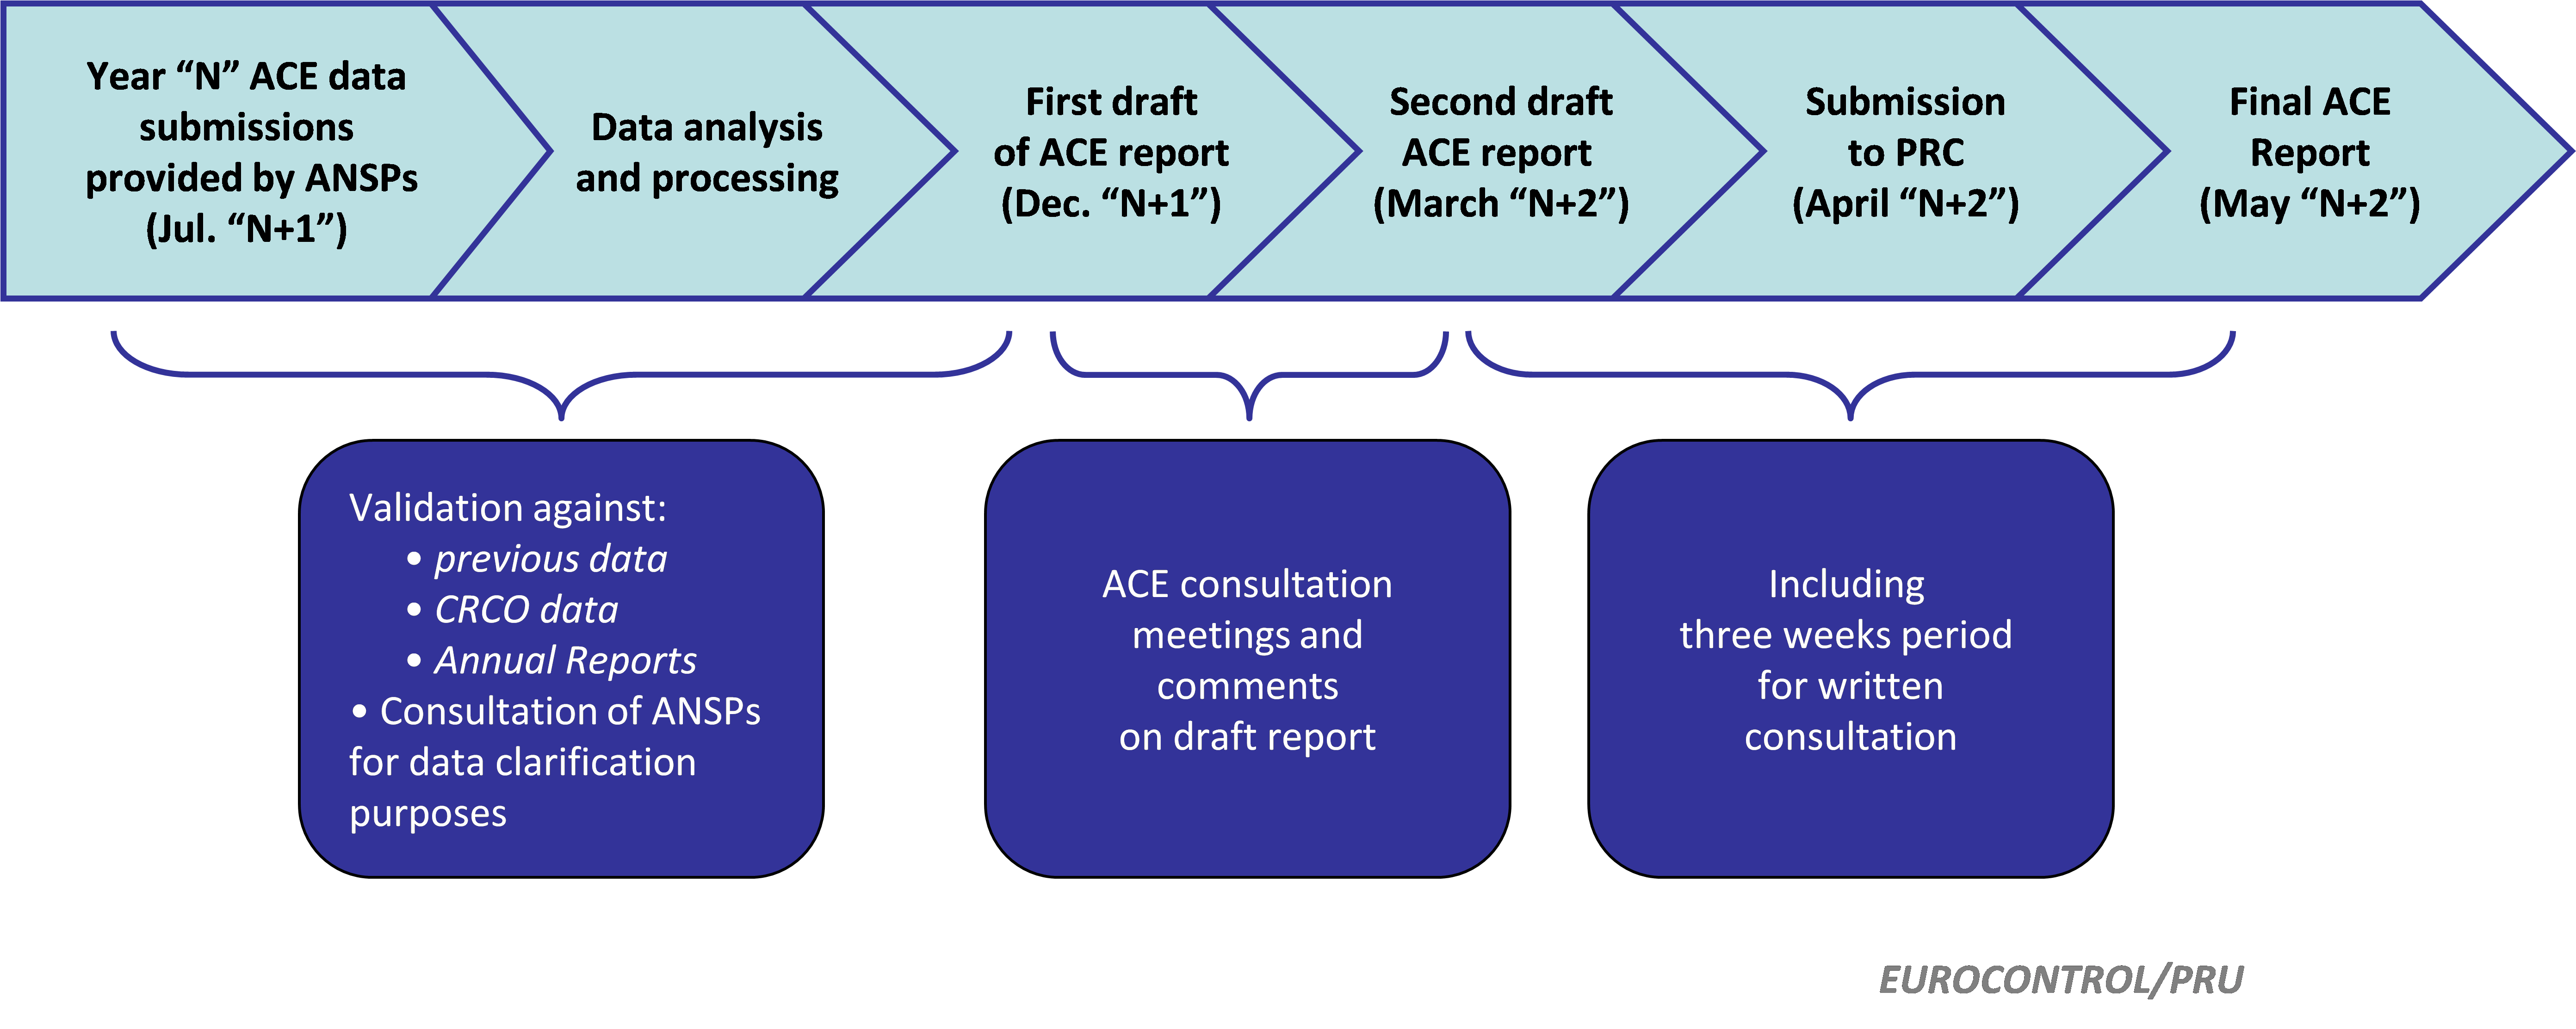
\includegraphics[width=1\linewidth,height=\textheight,keepaspectratio]{images/image2.png}

}

\caption{\label{fig-process}Data analysis, processing and reporting}

\end{figure}%

In order to ensure comparability among ANSPs and the quality of the
analysis, the information submitted by the ANSPs is subject to a
thorough analysis and verification process which makes extensive use of
ANSPs' Annual Reports and of their statutory financial accounts.

During this process a number of issues can emerge:

\begin{itemize}
\item
  Annual Reports with disclosure of financial accounts are not available
  for some ANSPs (see Section~\ref{sec-annual-report} below). This
  removes one important element in view of validating the financial data
  submitted.
\item
  ANSPs which are involved in non-ANS activities (such as airport
  ownership and management) do not necessarily disclose separate
  accounts for their ANS and non-ANS activities. This means that the
  financial data submitted for the ANS activities cannot be validated
  with the information provided in the Annual Report.
\item
  Except for a few ANSPs, Annual Reports do not disclose the separate
  costs for the various segments of ANS (such as en-route and terminal
  ANS) which means that the cost breakdown provided under the En-route
  and Terminal columns in the ACE data submissions cannot be fully
  reconciled.
\end{itemize}

As ANSPs progressively comply with the SES Regulation on Service
Provision (\citeproc{ref-ec550ux2f2004}{European Parliament and Council
of the European Union 2004}), which requires publication of Annual
Reports including statutory accounts, and separation of ANS from non-ANS
activity in ANSPs internal accounts, some of these shortcomings are
expected to be gradually overcome.

In most cases, data recorded in the Network Manager (NM) database are
used as the basis for the output metrics of the ACE data analysis.

\section{ANSPs' Annual Reports}\label{sec-annual-report}

ANSPs' Annual Reports provide a valuable means of validating the ACE
data.

The SES Service Provision Regulation
(\citeproc{ref-ec550ux2f2004}{European Parliament and Council of the
European Union 2004}) came into force on 20 April 2004 and is applicable
to ANSPs Financial Accounts in all EU Member States (plus Switzerland
and Norway). This Regulation is also applicable to States which have
signed the ECAA agreement or a Common Aviation Area agreement with the
European Union, although the timing of its implementation is not yet
decided for individual States. Among other provisions, the SPR requires
that ANSPs meet certain standards of information disclosure
(transparency) and reporting, and in particular that:

\begin{itemize}
\item
  ANSPs should draw up, submit to audit and publish their Financial
  Accounts (Art.12.1);
\item
  in all cases, ANSPs should publish an Annual Report and regularly
  undergo an independent audit (Art 12.2); and,
\item
  ANSPs should, in their internal accounting, identify the relevant
  costs and income for ANS broken down in accordance with EUROCONTROL's
  principles for establishing the cost-base for route facility charges
  and the calculation of unit rates and, where appropriate, shall keep
  consolidated accounts for other, non-air navigation services, as they
  would be required to do if the services in question were provided by
  separate undertakings (Art 12.3). The latter requirement is
  particularly relevant for the ANSPs which are part of an organisation
  which owns, manages and operates airports, such as HCAA and
  DHMI\footnote{Although it should be noted that DHMI is not covered by
    the SES regulations.}.
\end{itemize}

\bookmarksetup{startatroot}

\chapter{Methodological framework used to measure ANSPs gate-to-gate
cost-effectiveness performance}\label{sec-method}

\section{Composite output metric and framework for cost-effectiveness
performance analysis}\label{sec-metric-and-framework}

The output measures for ANS provision are, for en-route, the en-route
flight-hours controlled\footnote{Controlled flight-hours are calculated
  by the Network Manager (NM) as the difference between the exit time
  and entry time of any given flight in the controlled airspace of an
  operational unit. Three types of flight-hours are currently computed
  by the NM (filed model, regulated model and current model). The data
  used for the cost-effectiveness analysis is based on the current model
  (Model 3 or CFTM) and includes flight-hours controlled in the ACC, APP
  and FIS operational units which are described in the NM environment.}
and, for terminal ANS, the number of IFR airport movements controlled.
In addition to those output metrics, it is important to consider a
``gate-to-gate'' perspective, because the boundaries used to allocate
costs between en-route and terminal ANS vary between ANSPs and might
introduce a bias in the cost-effectiveness analysis.

For this reason, an indicator combining the two separate output measures
for en-route and terminal ANS provision has been calculated. The
``composite gate-to-gate flight-hours'' are determined by weighting the
output measures by their respective average cost of the service for the
whole Pan-European system.

This average weighting factor is based on the total monetary value of
the outputs over a period starting in 2002 and ending in the year under
review. The weighting factor can therefore vary marginally each time new
costs and traffic data are added to the ACE database. As an indication,
the value of the weighting factor based on the ACE 2023 data was around
0.28. However, composite flight-hours are calculated without rounding
this factor. ANSPs wishing to calculate the exact value of their
composite flight-hours can contact the PRU to get the exact figure,
without rounding.

The composite gate-to-gate flight-hours are consequently defined as:

\[ \textrm{Composite gate-to-gate flight-hours} = \textrm{En-route flight-hours} + (0.28 * \textrm{IFR airport movements}) \]

In the ACE 2001-2006 Reports (\citeproc{ref-ace_reports}{Performance
Review Unit 2023}), two different weighting factors were used to compute
ANSPs cost-effectiveness: one for the year under study and another to
examine changes in performance across time. As the ACE data sample
became larger in terms of years, the difference between these two
weighting factors became insignificant. For the sake of simplicity, it
was therefore proposed in the ACE 2007 benchmarking report to use only
one weighting factor to analyse ANSPs performance for the year and to
examine historical changes in cost-effectiveness.

Although the composite gate-to-gate output metric does not fully reflect
all aspects of the complexity of the services provided, it is
nevertheless the best metric currently available for the analysis of
gate-to-gate cost-effectiveness\footnote{Further details on the
  theoretical background to producing composite indicators can be found
  in a working paper on ``\emph{Total Factor Productivity of European
  ANSPs: basic concepts and application}'' (Sept.~2005)
  (\citeproc{ref-prc01ux2f2005}{Performance Review Commission 2005}).}.

For the sake of completeness, the gate-to-gate financial
cost-effectiveness indicator is broken down into en-route and terminal
components, with the output units being en-route flight-hours and IFR
airport movements, respectively. There are cases where a high en-route
cost per flight-hour correspond to a low terminal cost per IFR airport
movement and vice versa.

The PRU has developed an analytical framework that allows
cost-effectiveness to be broken down into a number of key components.
This framework helps in understanding differences in cost-effectiveness
by allowing examination of the detailed factors underlying it. It is
important to note that the focus of the ACE analysis is on the ATM/CNS
provision costs incurred by the ANSP. MET costs, EUROCONTROL costs and
States/NSAs costs are not included as not always under the ANSPs direct
management control.

\begin{figure}

\centering{

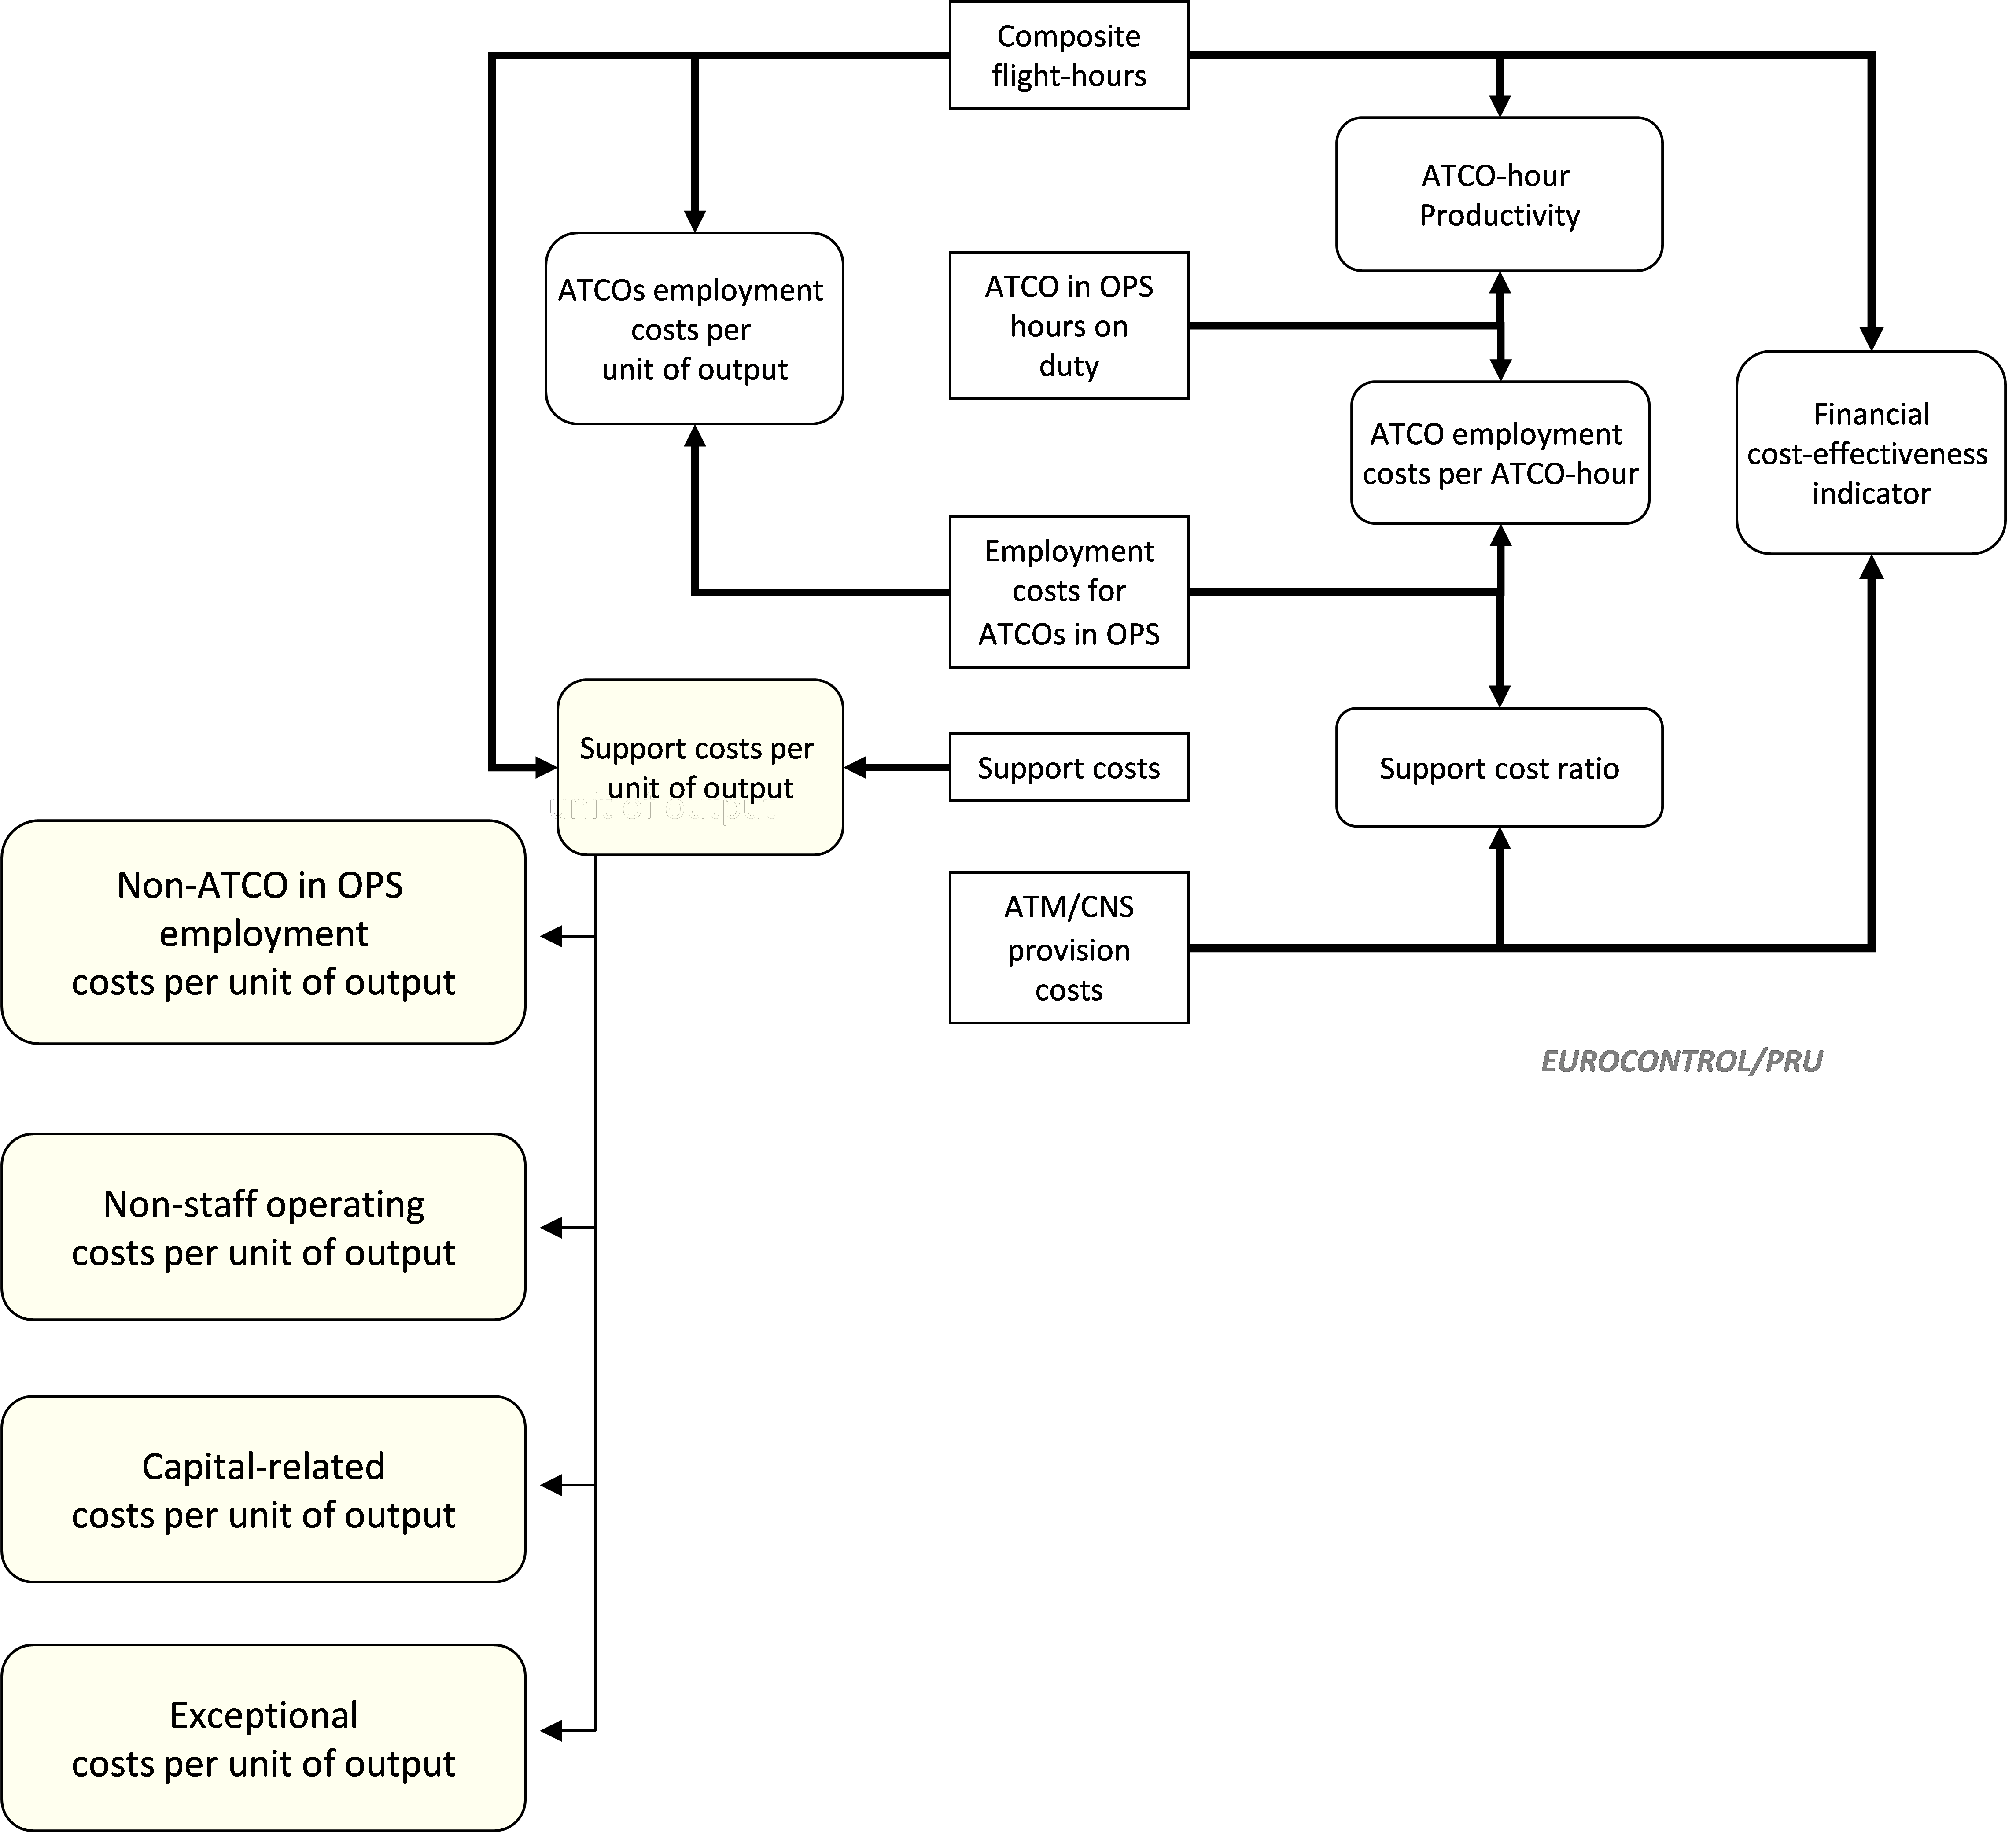
\includegraphics[width=1\linewidth,height=\textheight,keepaspectratio]{./images/image3.png}

}

\caption{\label{fig-framework-g2g}Performance framework for gate-to-gate
cost-effectiveness analysis}

\end{figure}%

The right-hand side of the Figure~\ref{fig-framework-g2g} shows that the
financial cost-effectiveness indicator (ATM/CNS provision costs per
composite flight-hour) is made up of three component performance
\textbf{ratios}:

\begin{itemize}
\item
  Higher ATCO-hour productivity (composite flight-hours per ATCO-hour)
  improves cost-effectiveness;
\item
  Lower ATCO \textbf{employment costs per ATCO-hour} improve
  cost-effectiveness; and,
\item
  All other things being equal, a lower \textbf{support cost ratio}
  improves cost-effectiveness.
\end{itemize}

These three ratios multiplied together give the overall financial
cost-effectiveness KPI.

The financial cost-effectiveness indicator can also be broken down into
two additive factors:

\begin{itemize}
\item
  \textbf{ATCO employment costs per unit of output} is the ratio of the
  employment costs for the ATCOs in OPS to the output (measured in
  composite flight-hours). All other things being equal, lower ATCOs in
  OPS employment costs per unit of output will improve financial
  cost-effectiveness.
\item
  \textbf{Support costs per unit of output} is the ratio of support
  costs to the output. All other things being equal, lower support costs
  per unit of output will improve financial cost-effectiveness.
\end{itemize}

The latter indicator is preferred to the support cost ratio for two main
reasons. First, the support cost ratio cannot be viewed in isolation
since a low ratio may simply be a symptom of high ATCO employment costs.
Second, given that there are fixed costs in the provision of ATM/CNS
(such as infrastructure and ATM systems), ``support costs per unit of
output'' can give additional insights into the analysis of support costs
and scale effects.

\section{Further methodological considerations on ATCO-hour
productivity}\label{further-methodological-considerations-on-atco-hour-productivity}

The metric of ATCO-hour productivity used in the ACE report is measured
as the ratio between composite flight-hours and ATCO in OPS hours on
duty. It reflects the average productivity during a year for a given
ANSP and does not give an indication of the productivity at peak times
which can be substantially higher.

Large differences in ATCO-hour productivity are observed in the ACE
analyses. These differences should not be seen in isolation, but
together with other indicators such as ATCO employment costs and unit
support costs. In addition, many factors contribute to the observed
differences in ATCO-hour productivity. Some of these factors can be
associated with operational conditions (such as traffic complexity and
variability, the type of airspace under the ANSP responsibility or the
number of airports operated by the ANSP potentially including low
traffic tower operational units), legal and socio-economic conditions
(e.g.~general labour laws) and institutional issues (e.g.~regulatory
aspects and governance arrangements).

Other factors as yet unidentified (and not measured) such as the impact
of different operational concepts and processes, the operational
flexibility, could also affect ATCO productivity performance. There may
also be cultural and managerial differences. These elements would
deserve additional analysis in order to provide further insight on the
differences in ATCO productivity and identify best practices.

Changes in ATCOs in OPS hours on duty could arise from:

\begin{itemize}
\item
  Changes in the number of FTE ATCOs in OPS (caused by such factors as
  newly licensed ATCOs, normal retirement, activation of an early
  retirement scheme);
\item
  Changes in the number of hours on duty, through:

  \begin{itemize}
  \item
    Modification of the contractual working hours following a new labour
    agreement;
  \item
    Changes in the number of hours not on duty (for example, through an
    increase in average sickness or in refresher training time); or,
  \item
    Changes in overtime (where applicable).
  \end{itemize}
\end{itemize}

In the context of the yearly benchmarking activity, the ACE reports
analyse ANSPs' productivity, both in terms of a cross-section analysis
for the year under review and in terms of time series (usually a
six-year period). This medium-term perspective is particularly useful
for observing changes over time, given the specific characteristics of
the ANS industry, which usually requires a certain lead-time to develop
ATM systems and infrastructure.

Improvements in ATCO-hour productivity can result from more effective
OPS room management and by making a better use of existing resources,
for example through the adaptation of rosters (preferably
individually-based to enhance flexibility) and shift times, effective
management of overtime, and through the adaptation of sector opening
times to traffic demand patterns. Similarly, advanced ATM system
functionalities and procedures are drivers for productivity
improvements.

On the other hand, it is clear that some of the measures implemented by
an ANSP to provide extra capacity can have a negative impact on its
ATCO-hour productivity performance. This is, for example, the case of a
sector split which will allow the ANSP to create additional capacity in
its airspace at the expense of more ATCOs or ATCO-hours on duty required
to man the additional sector(s).

\section{Further methodological considerations on support
costs}\label{further-methodological-considerations-on-support-costs}

Contrary to ATCO employment costs, support costs encompass a variety of
cost items which require specific analysis. There is a general
acknowledgement that the Pan-European system has excessive support costs
due to its high level of operational, organisational, technical and
regulatory fragmentation.

Support costs can be broken down into four separate components that
provide further insight into the nature of support costs:

\begin{enumerate}
\def\labelenumi{\alph{enumi})}
\tightlist
\item
  \textbf{Employment costs for non-ATCO in OPS staff}; these cover ATCOs
  on other duties, trainees, technical support and administrative staff.
  These costs can be affected by the following factors:
\end{enumerate}

\begin{itemize}
\item
  Outsourcing of non-core activities (such as maintenance of technical
  equipment, and professional training) could transfer costs from this
  category to non-staff costs.
\item
  Research \& development policies may involve ATM systems either being
  developed in-house, or purchased off-the-shelf. In principle, either
  solution could lead to the most cost-effective outcome, depending on
  circumstances; this would depend on whether there were, for example,
  significant economies of scale, or major transaction costs.
\item
  Arrangements relating to the collective agreement and the pension
  scheme for non-ATCOs in OPS.
\end{itemize}

\begin{enumerate}
\def\labelenumi{\alph{enumi})}
\setcounter{enumi}{1}
\tightlist
\item
  \textbf{Non-staff operating costs} mostly comprise expenses for
  energy, communications, contracted services, rentals, insurance, and
  taxes. These costs can be affected by the following factors:
\end{enumerate}

\begin{itemize}
\item
  The terms and conditions of contracts for outsourced activities.
\item
  Enhancement of the cooperation with other ANSPs to achieve synergies
  (sharing training of ATCOs, joint maintenance, and other matters).
\end{itemize}

\begin{enumerate}
\def\labelenumi{\alph{enumi})}
\setcounter{enumi}{2}
\tightlist
\item
  \textbf{Capital-related costs} comprising depreciation and financing
  costs for the capital employed. These costs can be affected by the
  following factors:
\end{enumerate}

\begin{itemize}
\item
  The magnitude of the investment programme.
\item
  The accounting life of the assets.
\item
  The degree to which assets are owned or rented.
\end{itemize}

\begin{enumerate}
\def\labelenumi{\alph{enumi})}
\setcounter{enumi}{3}
\tightlist
\item
  \textbf{Exceptional costs}, which typically represent a very small
  proportion of support costs.
\end{enumerate}

There are significant differences in the composition of support costs
amongst the 38 ANSPs, and in particular in the proportion of employment
costs and non-staff operating costs. The choice between providing some
important operational support functions internally or externally has
clearly an impact on the proportion of support costs that is classified
as employment costs, non-staff operating costs, or capital-related
costs. In some cases, the maintenance of ATM systems is outsourced and
the corresponding costs are reported as non-staff operating costs. For
other ANSPs, these activities are rather carried out by internal staff
and the related costs appear as employment costs or as capital-related
costs when, according to IFRS, the employment costs of staff working on
R\&D projects can be capitalised in the balance-sheet.

Employment costs are typically subject to complex bargaining agreements
between ANSPs management and staff which usually are embedded into a
collective agreement. The duration of the collective agreement, the
terms and methods for renegotiation greatly vary across ANSPs. In some
cases salary conditions are negotiated every year. High ATCO employment
costs may be compensated for by high productivity. Therefore, in the
context of staff planning and contract renegotiation, it is important
for ANSPs to manage ATCOs employment costs effectively and to set
quantitative objectives for ATCO productivity while providing sufficient
capacity in order to minimise ATFM delays.

\bookmarksetup{startatroot}

\chapter{ATFM delays and cost-effectiveness
performance}\label{sec-delay-cef}

The quality of service provided by ANSPs has an impact on the efficiency
of aircraft operations, which carry with them additional costs that need
to be taken into consideration for a full economic assessment of ANSP
performance. In the ACE benchmarking reports, an indicator of
``economic'' cost-effectiveness is computed at ANSP and Pan-European
system levels by adding the ATM/CNS provision costs and the costs of
ATFM ground delay, all expressed per composite flight-hour.

\begin{figure}

\centering{

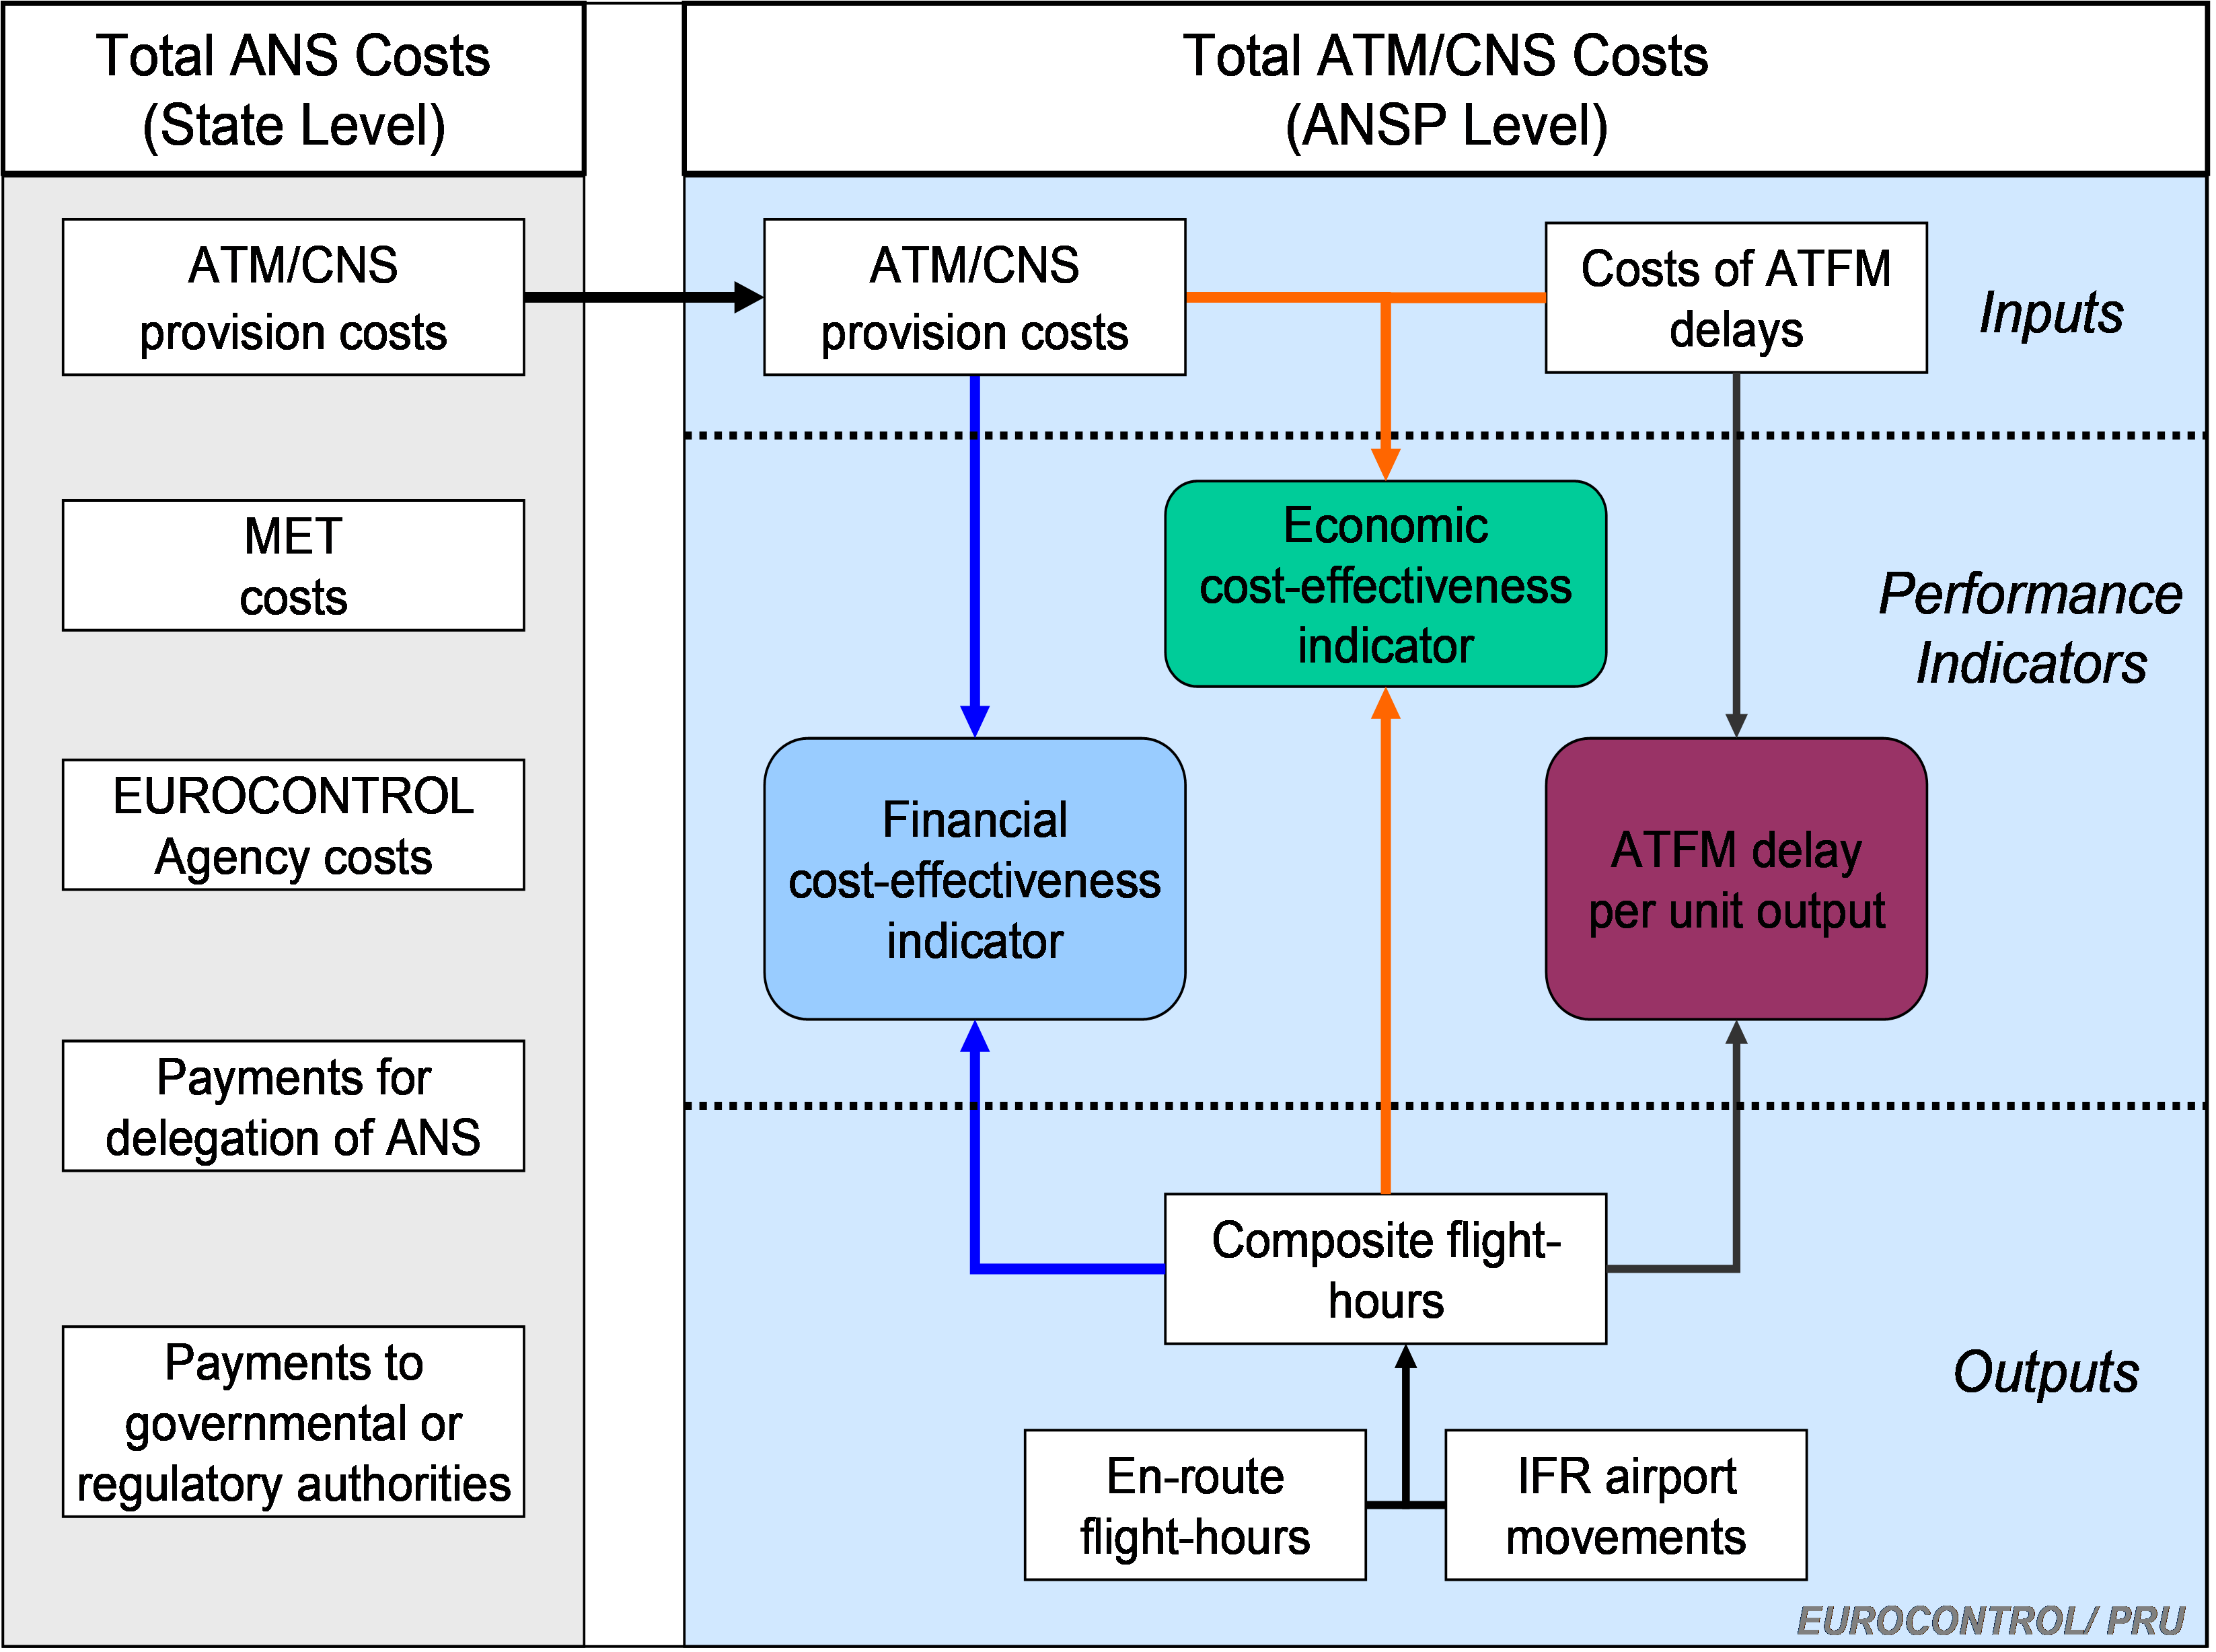
\includegraphics[width=1\linewidth,height=\textheight,keepaspectratio]{./images/image4.png}

}

\caption{\label{fig-framework-economic}Framework for economic
cost-effectiveness performance analysis}

\end{figure}%

ATFM delays used in the ACE analysis are extracted from the Network
Manager database. All delay causes (e.g.~capacity, weather, etc.) are
considered.

Only airports where the ANSPs are responsible to provide ATC services
are taken into account when aggregating airport delays at ANSP level.
This is verified each year during the ACE data validation process.
Airport ATFM delays also include departure delays.

ATFM delays are calculated after post-ops and eNM adjustments, which
entails a re-allocation of ATFM delays across ACCs in order to account
for the initiatives taken to improve performance at network level. This
process was initially launched in 2016 but the magnitude of ATFM delay
reallocation became really significant in 2018 and 2019 due to the large
extent of the measures implemented by the NM. In order to have
consistent time series within the ACE report, the adjusted ATFM delays
are used retroactively starting from 2016.

Delays are taken into account independently of their duration. There is
no distinction between delays lower or higher than 15 minutes.

The cost of ATFM delay in this report is based on the \emph{European
airline delay cost reference values}, published by the University of
Westminster (\citeproc{ref-uow:costofdelay}{University of Westminster
2015}). In each new ACE report, the PRU expresses the cost of one minute
of ATFM delay in the price base of the year under review, using the
average European Union inflation rate published by EUROSTAT.

\bookmarksetup{startatroot}

\chapter{Factors affecting
performance}\label{factors-affecting-performance}

\section{Introduction}\label{introduction-1}

The ACE benchmarking analysis has the objective of comparing ATM
cost-effectiveness performance across a wide range of ANSPs. The major
focus of the ACE report is to examine and analyse the quantitative facts
about the observed cost-effectiveness performance of the ANSPs. This
factual analysis provides a comprehensive description and comparison of
performance as viewed by the users of ATM/CNS services.

However, such a factual analysis cannot be either a complete explanation
of performance differences between ANSPs, or an exhaustive guide on how
performance can be improved, without some complementary consideration of
how differences in performance arose.

The framework illustrated in Figure~\ref{fig-factors-cost} shows
\textbf{exogenous} (outside the control of ANSPs) and
\textbf{endogenous} (under ANSPs' control) factors which influence ANSP
performance.

\begin{figure}

\centering{

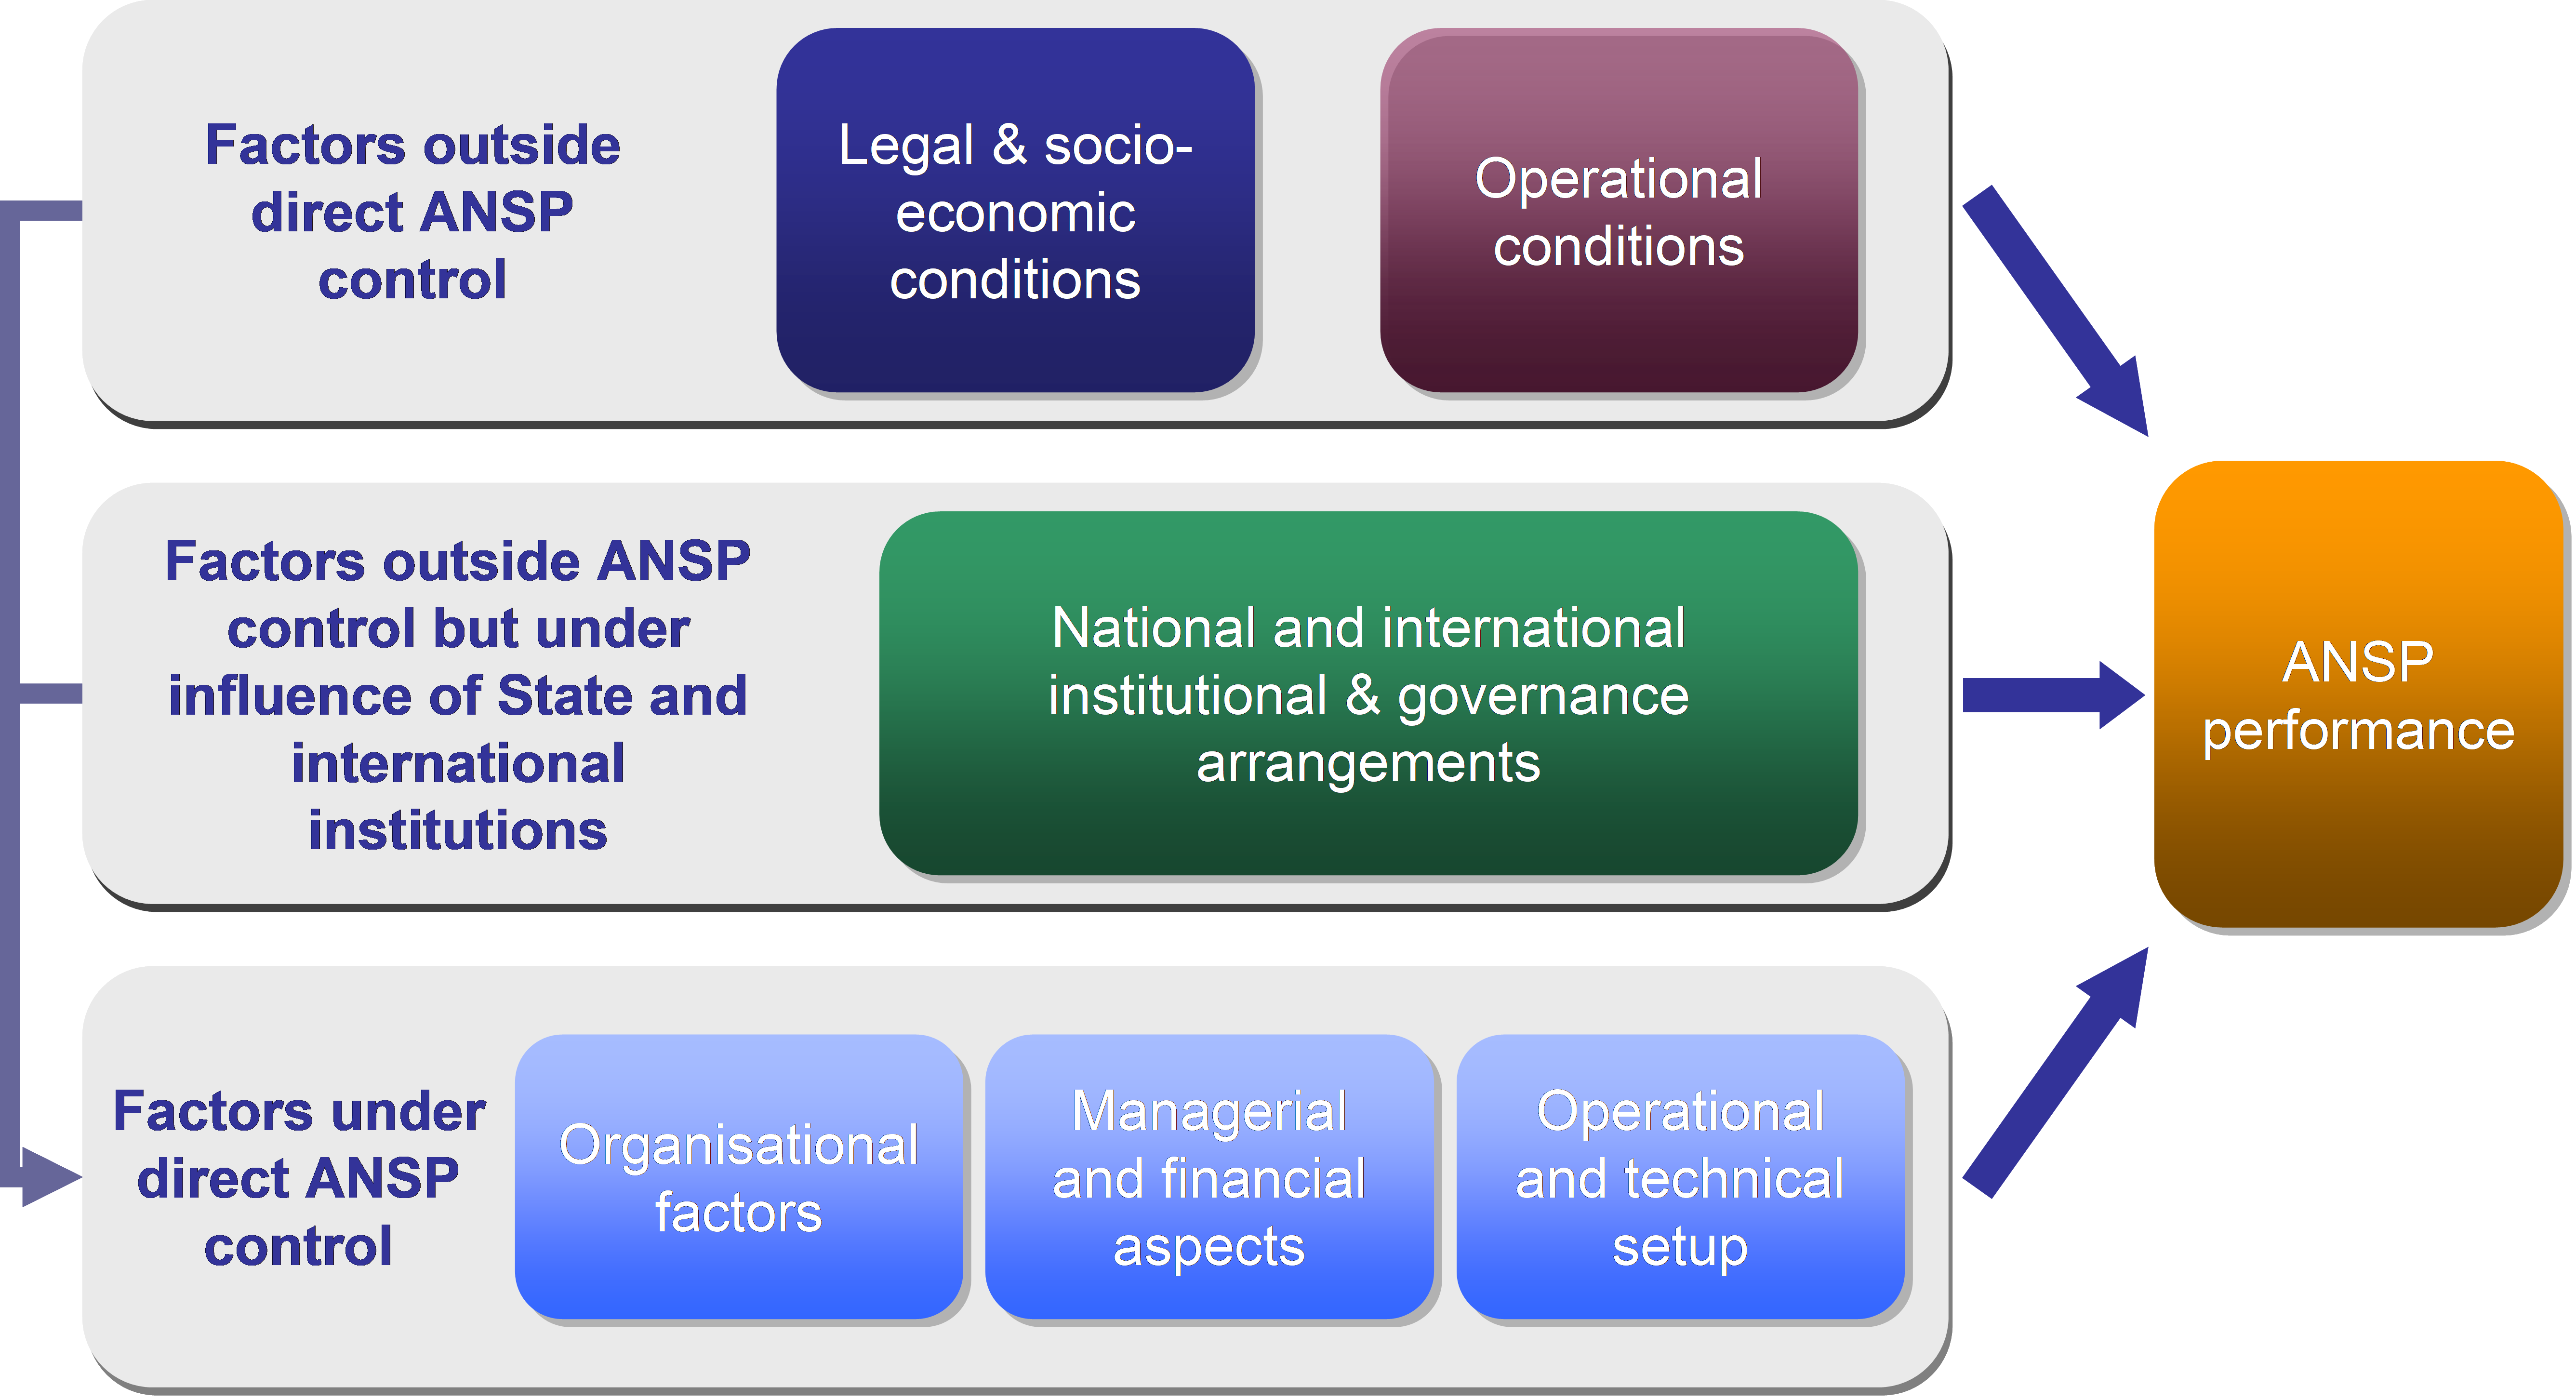
\includegraphics[width=0.8\linewidth,height=\textheight,keepaspectratio]{./images/image5.png}

}

\caption{\label{fig-factors-cost}Factors affecting cost-effectiveness
performance}

\end{figure}%

\section{Exogenous factors}\label{exogenous-factors}

Exogenous factors arise from the basic conditions in which an ANSP
operates, which can differ from one country to another. Exogenous
factors are likely to influence the way ANSPs organise and conduct their
business. In some cases they may also affect the way an ANSP manages
costs and determines the level of charges.

Exogenous factors cover a spectrum of observability and measurability.
At one extreme, the impact of irrecoverable VAT on inputs, which differs
from state to state, is readily quantified. It has a direct impact on
apparent performance which can be perfectly adjusted for. At an
intermediate level there are factors for which it is possible to derive
metrics (examples are traffic complexity, market wage rates, and
exchange rate volatility), but it is difficult to specify exactly how
such factors might affect performance. Even more difficult to take into
account are factors such as political influence (and interference) on
ANS provision. Finally, there will inevitably be exogenous factors that
are simply impossible to identify, although they are no less real than
the other factors discussed.

In Figure~\ref{fig-factors-cost}, exogenous factors that could have an
impact on performance have been classified into two main areas (top and
central set of factors in Figure~\ref{fig-factors-cost}), according to
which set of decision-makers have an influence over them. The top set,
comprising legal and socio-economic conditions, and operational
conditions, are affected by decision makers and conditions outside
aviation policy-making. The central set, comprising institutional and
governance arrangements, are exogenous to the ANSP but are influenced by
aviation sector policy decisions.

Exogenous factors need, as far as possible to be taken into account both
in achieving fair benchmarking, and in effective target setting:

\begin{itemize}
\item
  Local differences in exogenous factors can either create a direct
  advantage or a direct burden on performance;
\item
  Local institutional and governance arrangements may have been set with
  the specific purpose of creating incentives to follow
  performance-driven strategies.
\end{itemize}

Capturing the local impact of an exogenous factor on ANSPs performance
is not a straightforward exercise. First, there is no guarantee that a
given exogenous factor will affect all ANSPs in the same manner. It is
possible that similar conditions could create effects working in
opposite direction (bringing both benefits and difficulties). Second,
similar exogenous factors may not necessarily affect different ANSPs to
the same degree, either because of endogenous factors relating to how an
issue is managed, or by other exogenous factors constraining an ANSP's
response. So a given factor might create a small burden in one ANSP,
while affecting another more seriously.

The \textbf{legal and socio-economic conditions} prevailing in
individual countries are affected by national policy-makers at a more
general level (for example taxation policy), or by national and
international macro-economic conditions. Major examples include the
prevailing national wage rates, and levels and systems of taxation.

Some examples that affect ATM cost-effectiveness performance are
illustrated in Figure~\ref{fig-legal-socio}.

\begin{figure}[H]

\centering{

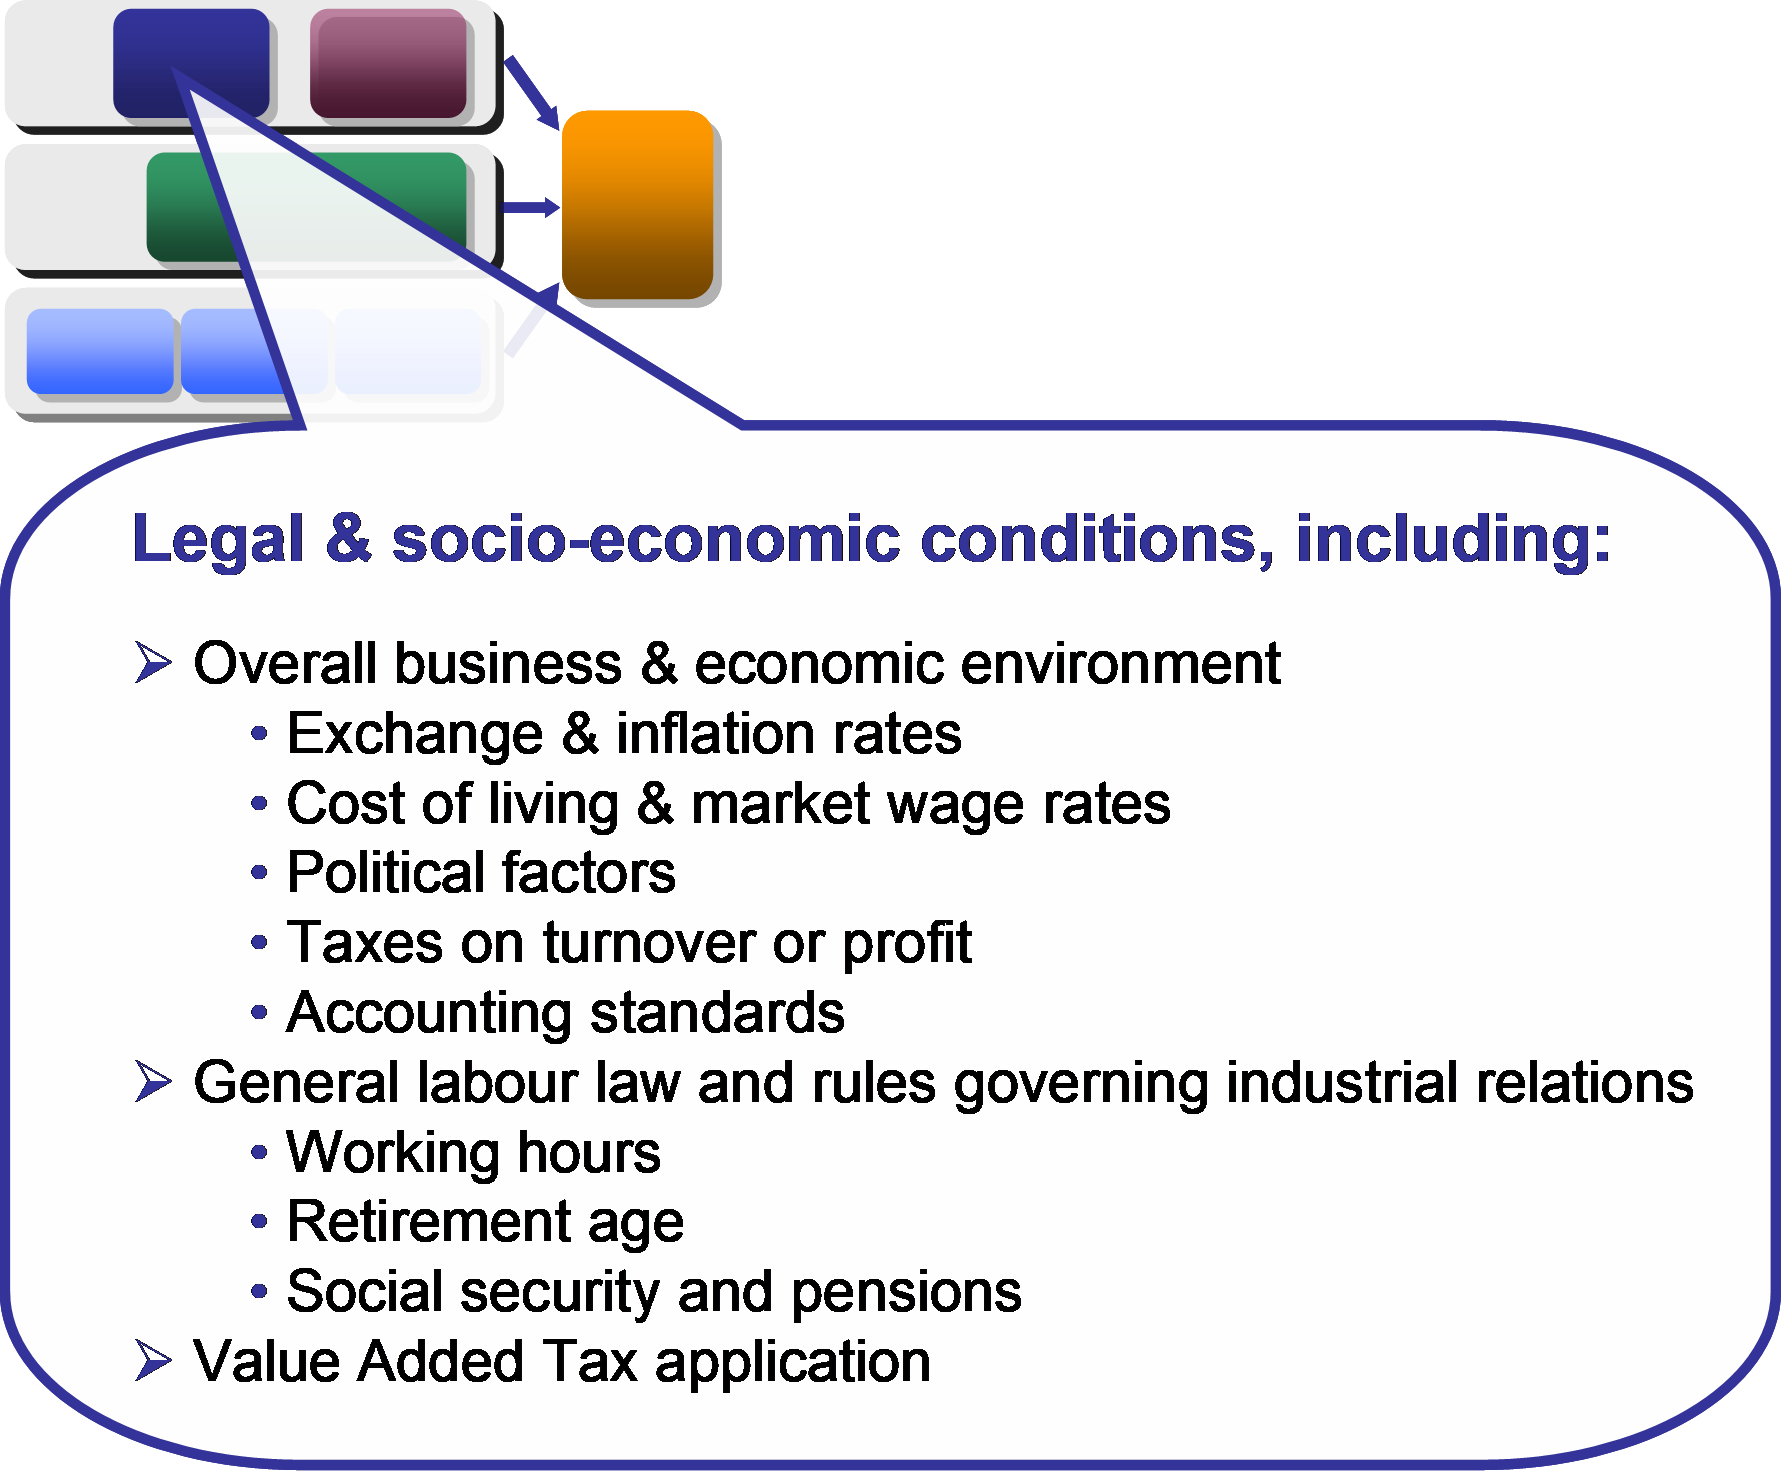
\includegraphics[width=0.6\linewidth,height=\textheight,keepaspectratio]{./images/image6.png}

}

\caption{\label{fig-legal-socio}Legal \& socio-economic conditions}

\end{figure}%

The \textbf{operational conditions}, such as the traffic patterns the
ANSP has to deal with, are determined by decisions made by airports,
airlines, and especially, flying travellers.

Operational conditions include a number of factors, summarised in
Figure~\ref{fig-operational-conditions}.

\begin{figure}[H]

\centering{

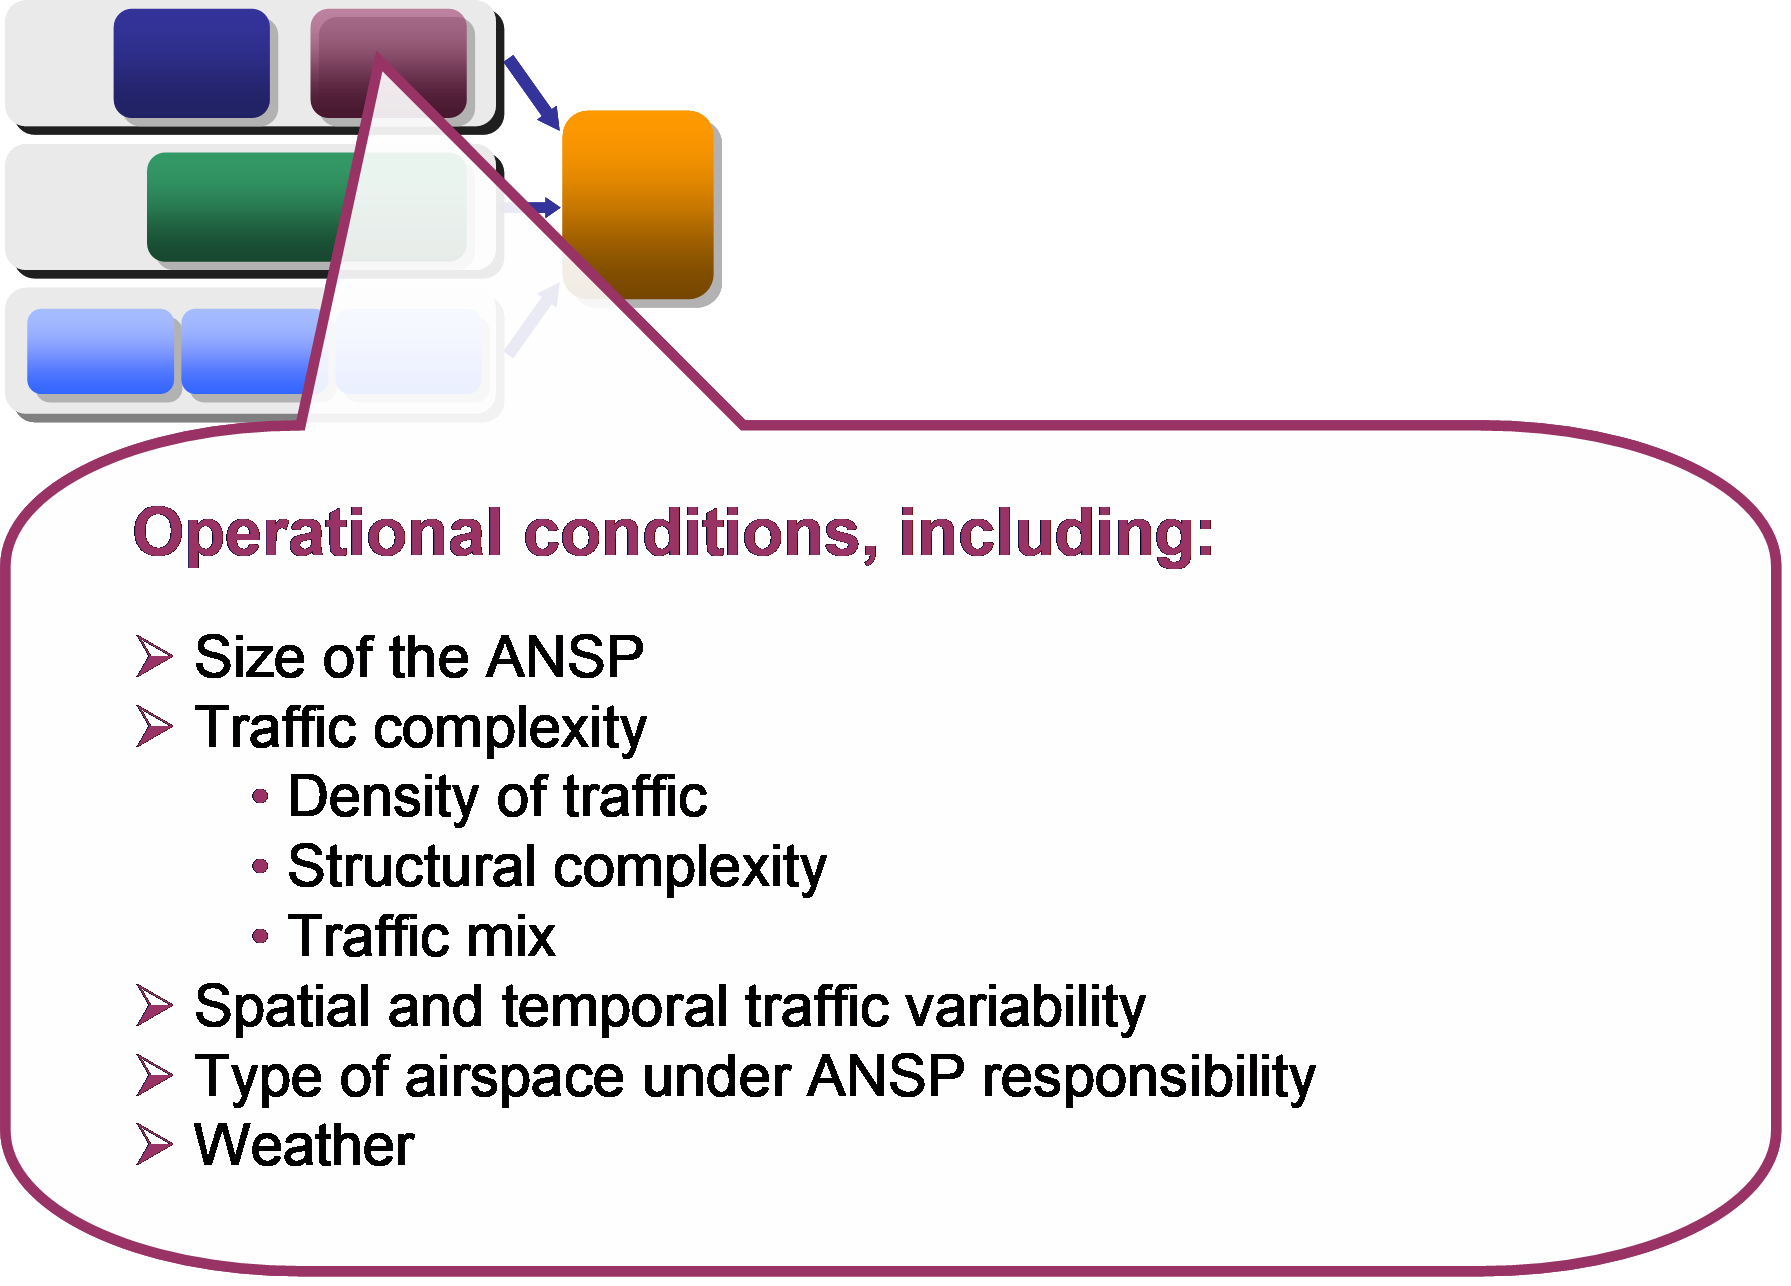
\includegraphics[width=0.6\linewidth,height=\textheight,keepaspectratio]{./images/image7.png}

}

\caption{\label{fig-operational-conditions}Operational conditions}

\end{figure}%

Operational conditions undoubtedly have a direct impact on
cost-effectiveness performance, although the extent and magnitude of the
impact is not straightforward to isolate.

The \textbf{institutional and governance arrangements} for ANS in a
particular country are set in place by the policies and specific
aviation laws of each country. These factors are exogenous to the ANSP
but decision-making concerning some of them is largely driven by
national aviation policy-makers. Some of these factors relate to
international requirements such as those imposed by ICAO, EUROCONTROL
and the Single European Sky. These policies at State and European level
are subject to changes given strategic objectives for the sector.

Figure~\ref{fig-institutional-arrangements} provides a list of such
factors, relating to:

\begin{itemize}
\tightlist
\item
  the way ANS is regulated;
\item
  the institutional structure surrounding ANS, the ANSP ownership and
  control structure; and
\item
  the civil/military arrangements.
\end{itemize}

\begin{figure}[H]

\centering{

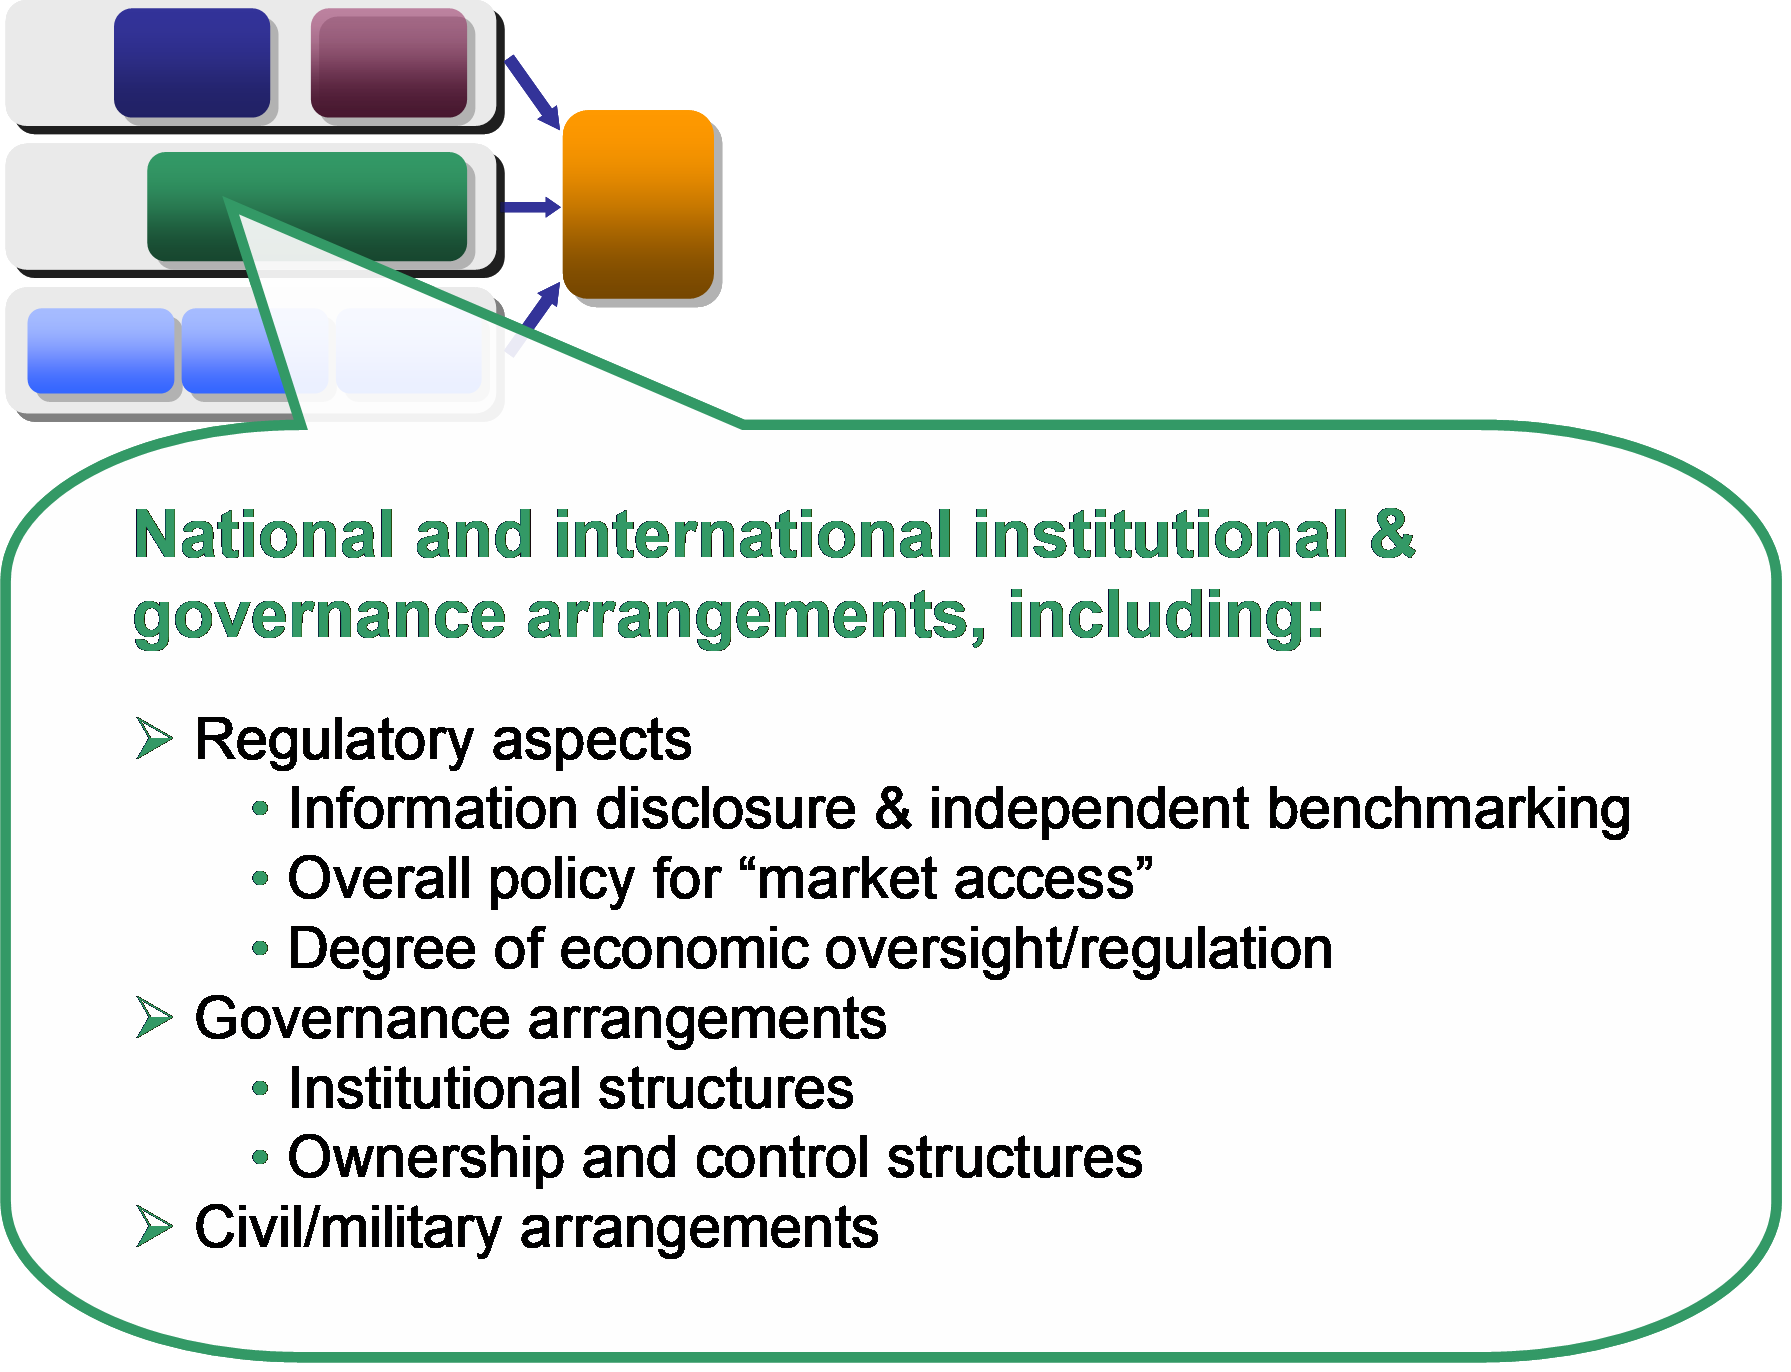
\includegraphics[width=0.6\linewidth,height=\textheight,keepaspectratio]{./images/image8.png}

}

\caption{\label{fig-institutional-arrangements}Institutional \&
governance arrangements}

\end{figure}%

It is generally considered that institutional and governance
arrangements will not affect ATM cost-effectiveness directly; rather
they act as influences or constraints affecting endogenous factors (such
as the overall business objectives, the internal organisation, and the
operational setup between civil and military).

\section{Endogenous factors}\label{endogenous-factors}

In principle, once the impact of all exogenous factors has been allowed
for, the performance differences that remain should comprise residual
inefficiency which lowers performance below that obtained by best
practice. Such residual inefficiency arises from a number of endogenous
factors, under the direct control of ANSPs.

A better understanding of the endogenous factors would enable some
progress in the analysis of benchmarking results, in the identification
of best practices, and in the process of target setting.

Endogenous factors -- the way that an ANSP manages its business to
optimise performance -- are influenced by exogenous factors. ``Best
practice'' in any given area will depend on the exogenous circumstances.
ANSPs can take action to fully exploit the benefit of their environment
or to minimize the impact of relative disadvantages. Therefore, the
impact of an exogenous factor should not be analysed in isolation from
an analysis of the degree to which this impact has been minimised or
maximized through appropriate internal measures.

Different data and methodologies from those currently used in the ACE
Benchmarking Report would be required to investigate endogenous factors
in more depth. Clearly, it is the responsibility of the ANSP to
determine how best to respond to the local conditions.

Endogenous factors fall into three groups:

\begin{itemize}
\tightlist
\item
  organisational factors;
\item
  managerial and financial aspects; and,
\item
  operational and technical setup.
\end{itemize}

Figure~\ref{fig-org-factors} lists the factors that would need to be
considered in the scope of a comprehensive analysis of the impact of
\textbf{ANSP organisation} on performance. They mainly relate to four
issues which are typically addressed in the Balanced Scorecard
methodology.

\begin{figure}[H]

\centering{

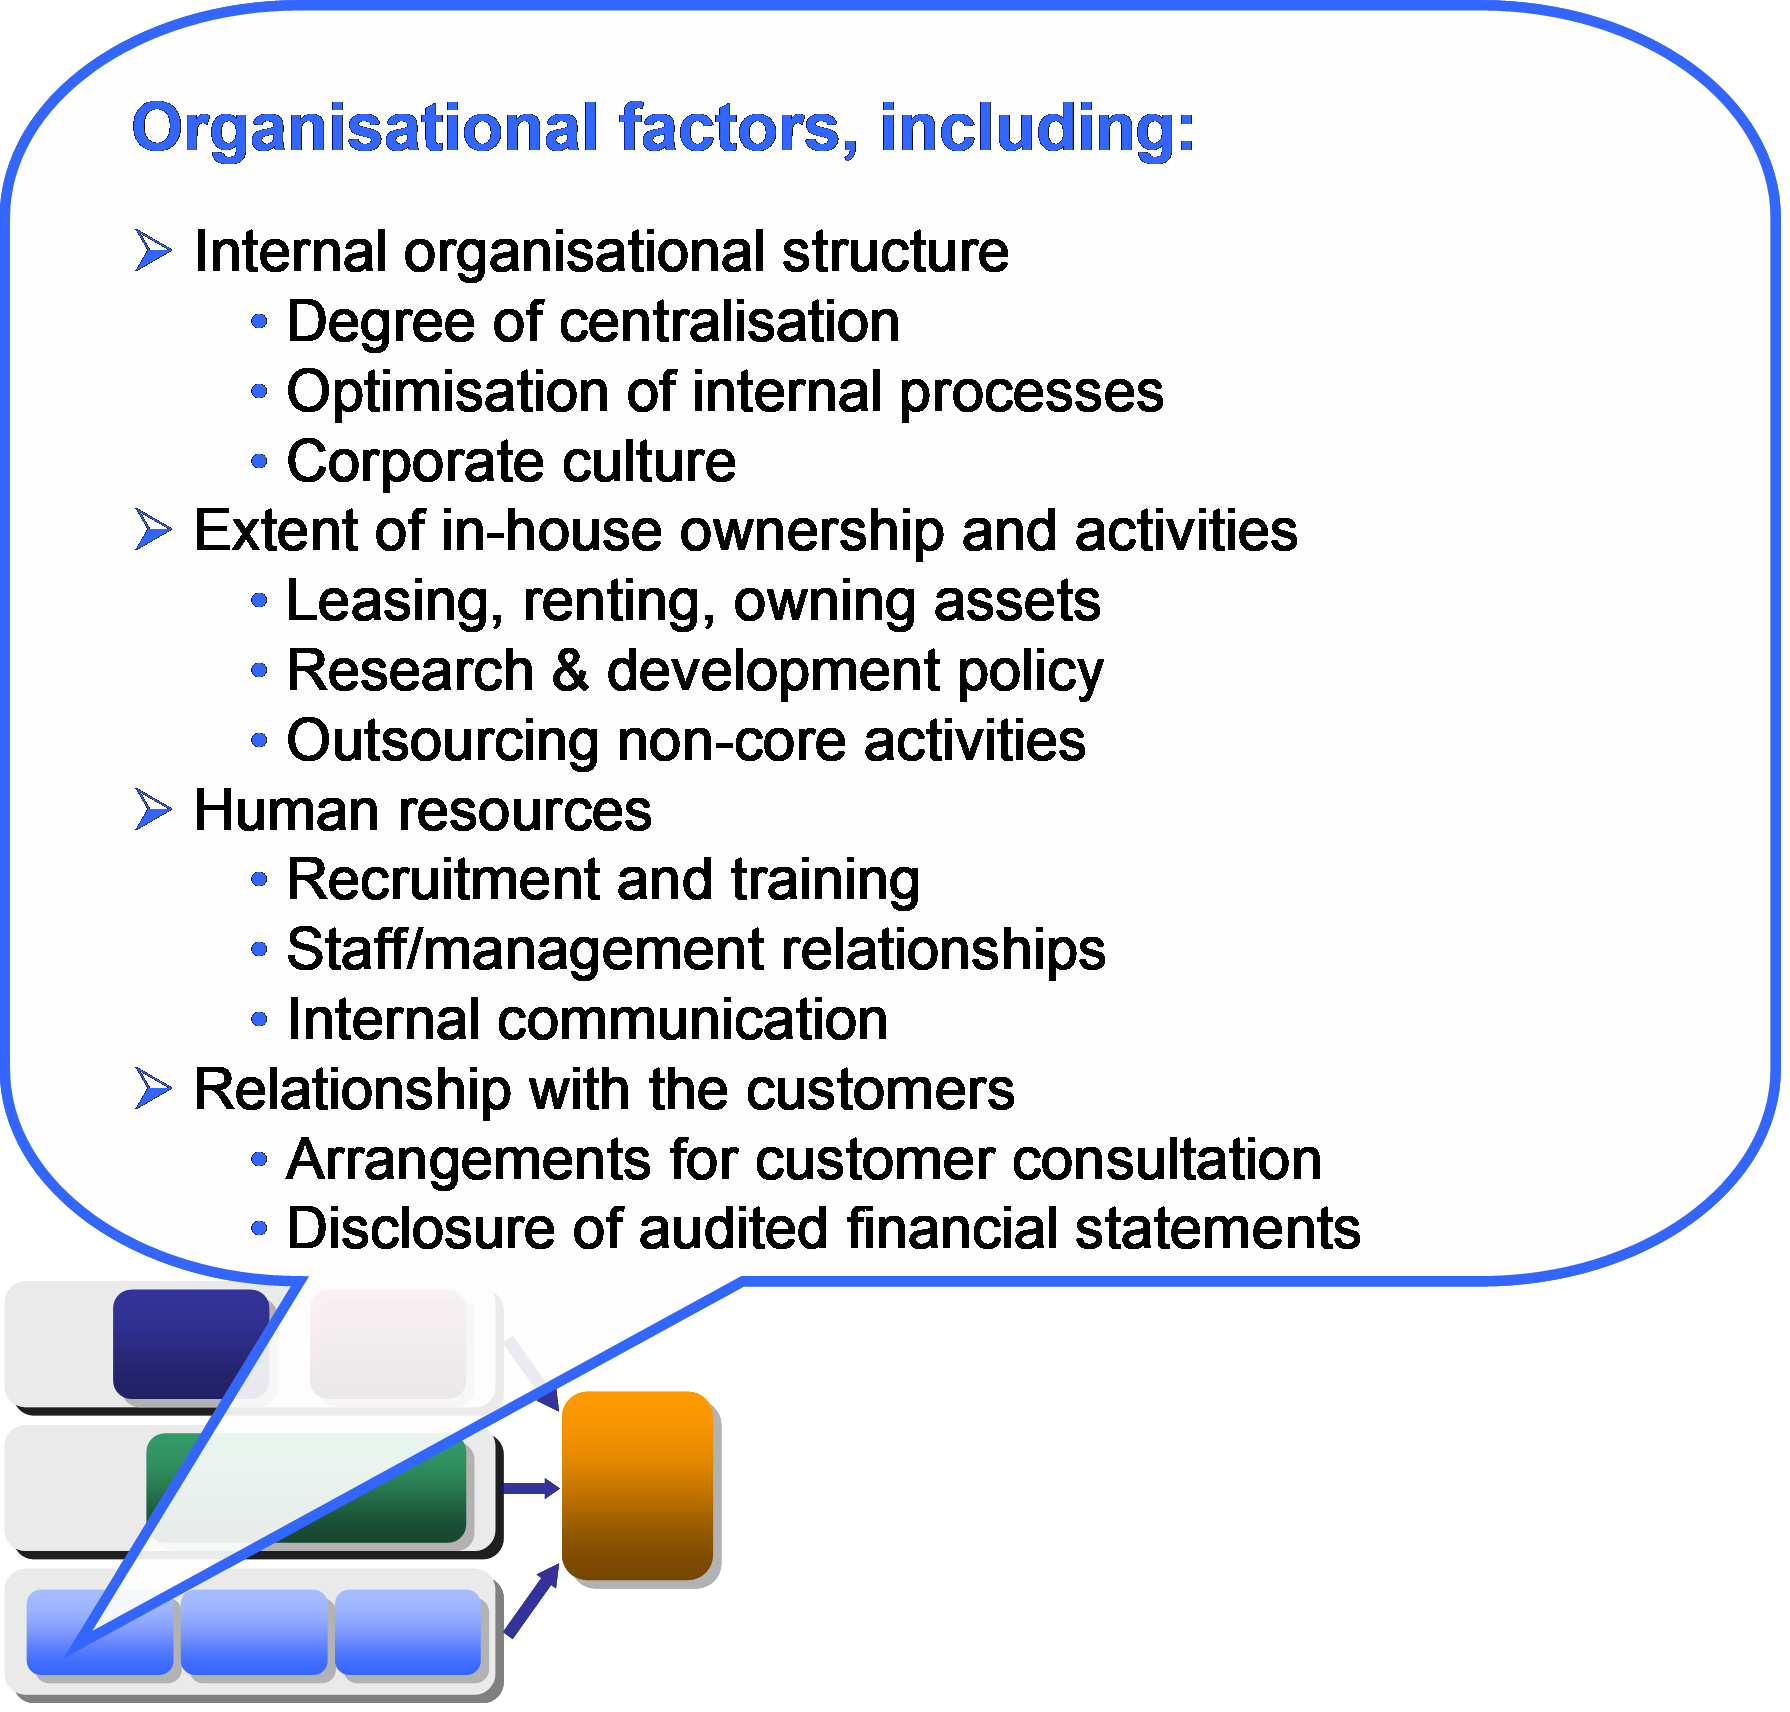
\includegraphics[width=0.55\linewidth,height=\textheight,keepaspectratio]{./images/image9.png}

}

\caption{\label{fig-org-factors}Organisational factors}

\end{figure}%

These issues are:

\begin{itemize}
\tightlist
\item
  The internal organisation structure;
\item
  The degree to which assets and activities are retained in-house;\\
\item
  Human resources; and\\
\item
  Relationship with customer.
\end{itemize}

Not all organisational factors will directly affect cost-effectiveness;
some enable or facilitate the achievement of performance when they are
set in conformity with the business objectives. It is likely that no
single model should constitute ``best practice'' in all circumstances.

Figure~\ref{fig-managerial} provides a list of factors that would need
to be considered in the scope of a comprehensive examination of the
influence of ANSP \textbf{managerial and financial arrangements} on
performance. They mainly relate to the following three issues:

\begin{itemize}
\tightlist
\item
  The quality of management;
\item
  The collective bargaining process; and
\item
  Financial and accounting considerations.
\end{itemize}

\begin{figure}[H]

\centering{

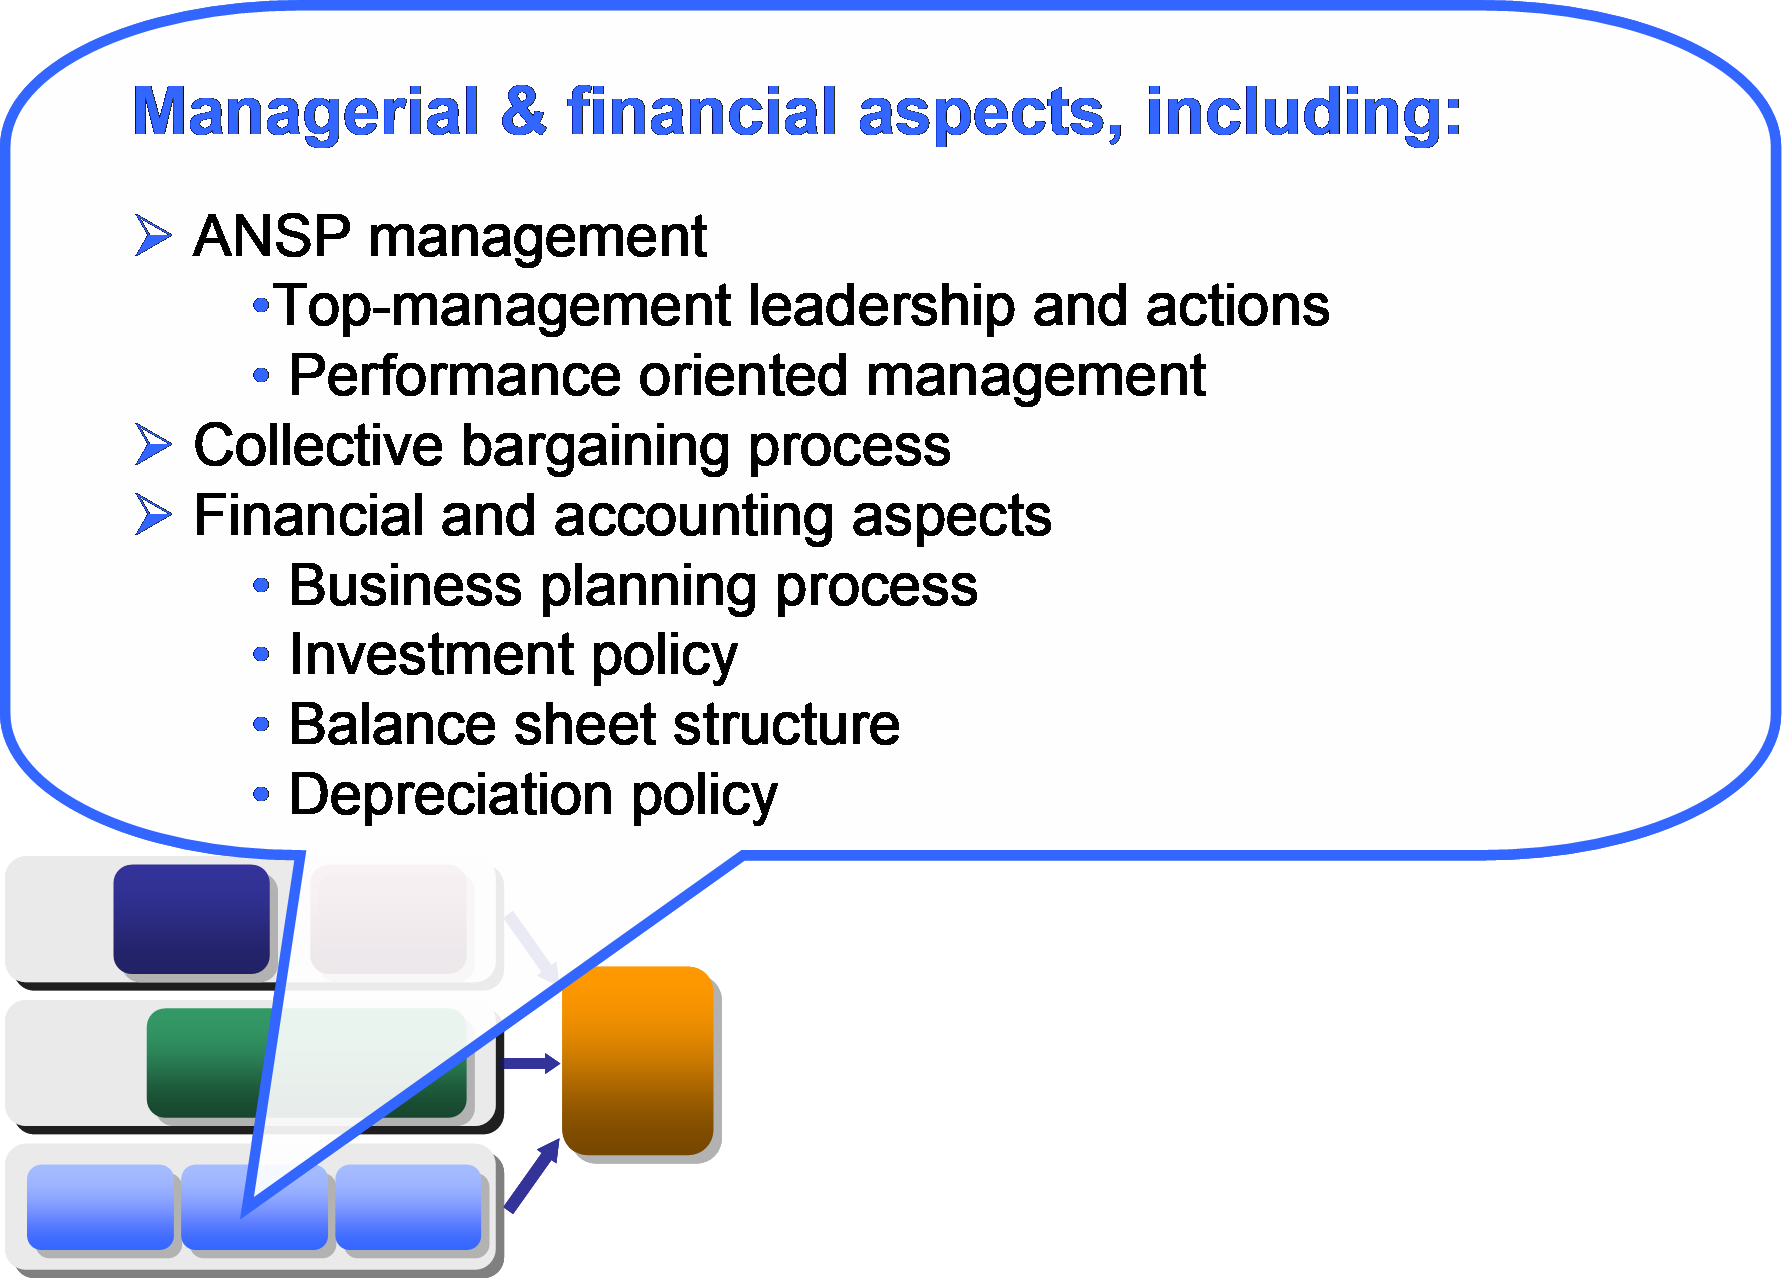
\includegraphics[width=0.55\linewidth,height=\textheight,keepaspectratio]{./images/image10.png}

}

\caption{\label{fig-managerial}Managerial \& financial aspects}

\end{figure}%

Most of the managerial and financial aspects are expected to directly
affect cost-effectiveness, since they have an impact, for example, on
investment decisions, productivity and wage policies. The managerial and
financial aspects are to some extent influenced by the ANSP
organisational factors and by some of the exogenous factors (especially
among the institutional and governance factors, and among the
socio-economic factors).

Figure~\ref{fig-operational-setup} provides a list of factors that would
need to be considered in a comprehensive examination of the influence of
\textbf{ANSP operational and technical setup} on performance. They
mainly relate to the following three issues:

\begin{itemize}
\tightlist
\item
  Operational structure;
\item
  Operational concepts and processes; and
\item
  Operational flexibility.
\end{itemize}

\begin{figure}[bht]

\centering{

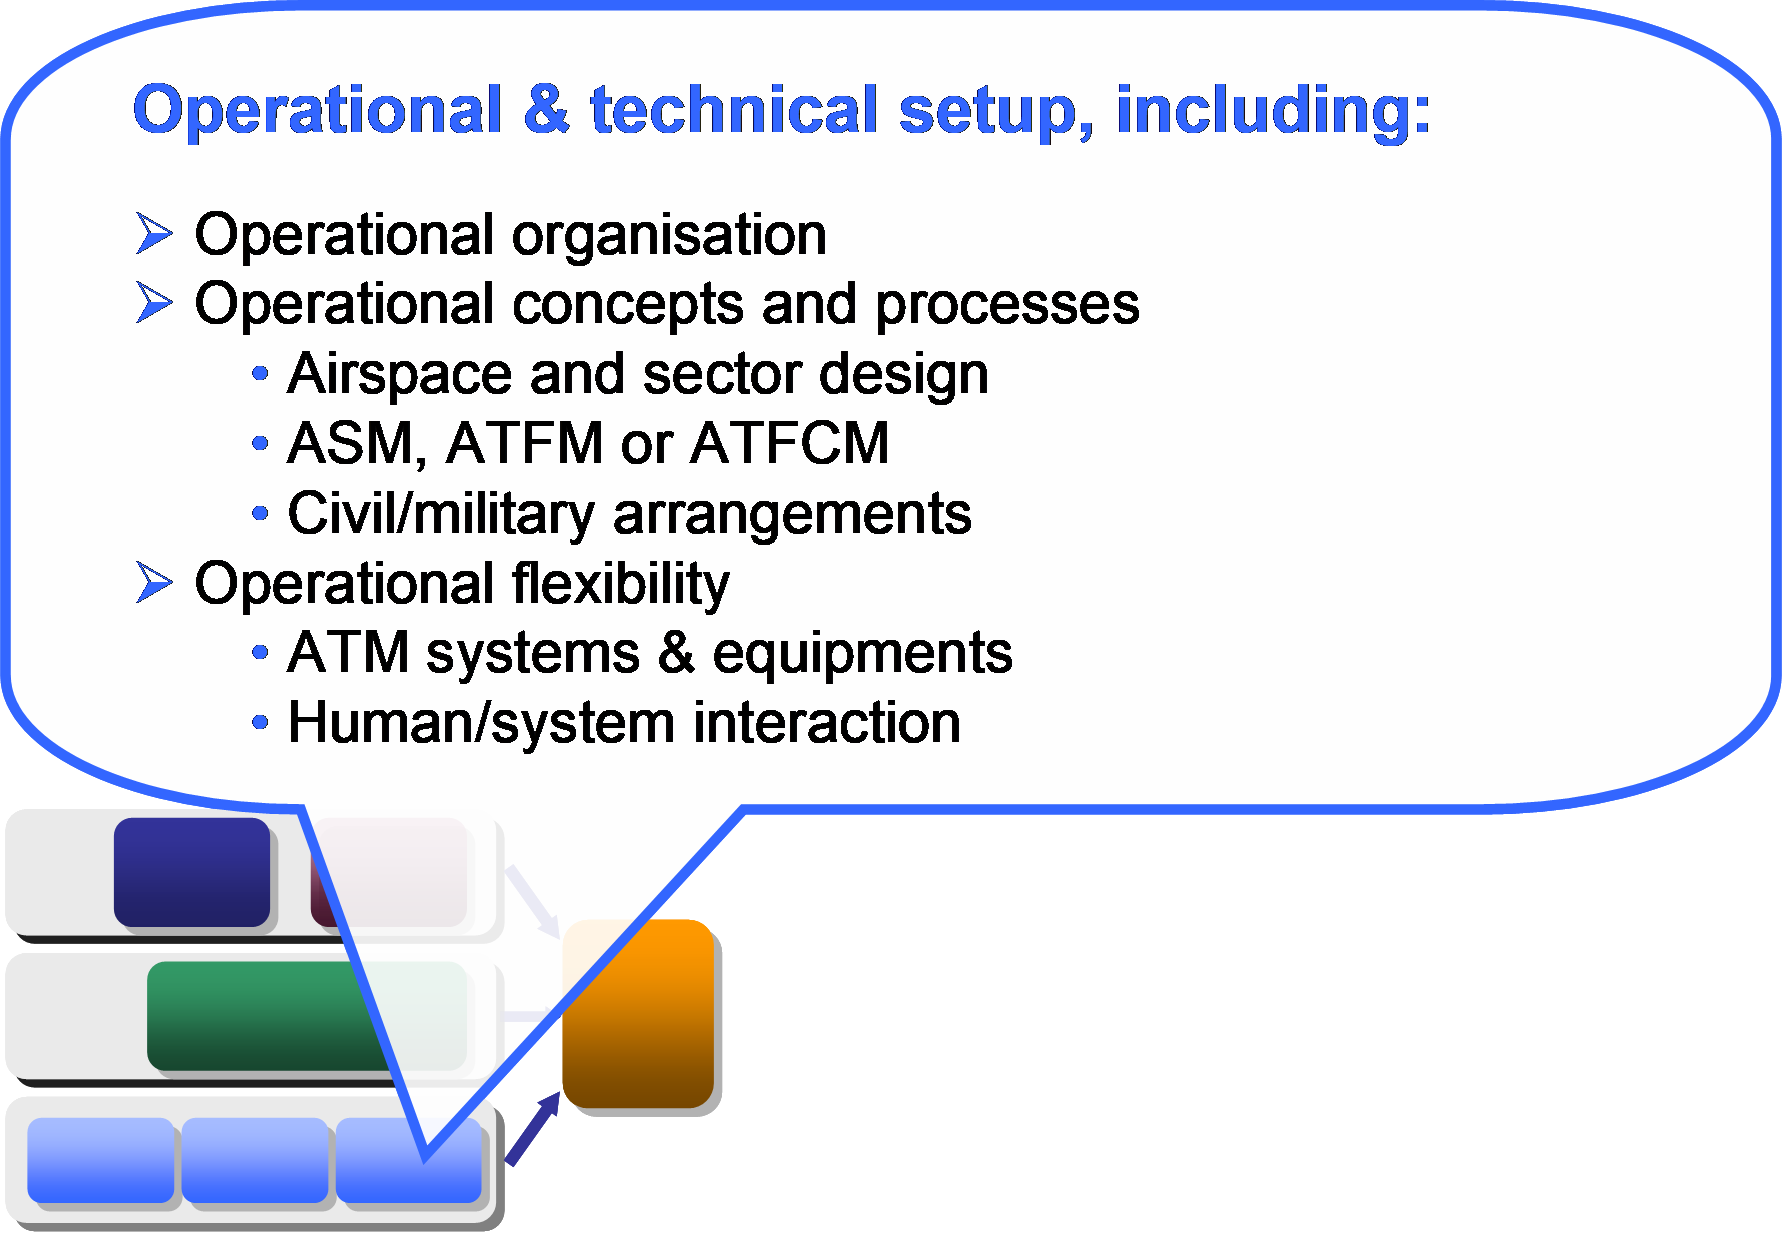
\includegraphics[width=0.6\linewidth,height=\textheight,keepaspectratio]{./images/image11.png}

}

\caption{\label{fig-operational-setup}Operational \& technical setup}

\end{figure}%

The operational and technical setup of an ANSP is expected to be
influenced by both exogenous factors (typically the operational
environment) and other endogenous factors (such as internal organisation
and investment policy). The operational and technical setup is expected
to affect both labour and capital productivity and the level of support
costs.

\bookmarksetup{startatroot}

\chapter{ANSP benchmarking and the SES Performance
Scheme}\label{ansp-benchmarking-and-the-ses-performance-scheme}

The objective of this chapter is to explain the main differences between
the ACE financial cost-effectiveness indicator and the Single European
Sky (SES) en-route cost-efficiency KPI (as defined in Regulation (EU)
N°2019/317 (\citeproc{ref-eu2019ux2f317}{European Commission 2019})).

First of all, it should be noted that these two indicators have been
specified in response to different needs:

\begin{itemize}
\item
  The purpose of the ACE analysis is to benchmark the cost-effectiveness
  performance of ANSPs in providing gate-to-gate ATM/CNS services (where
  en-route and terminal ATM/CNS are considered together). The ACE
  financial cost-effectiveness indicator is computed as the ratio of
  ATM/CNS provision costs to composite flight-hours and it can be broken
  down into three components (ATCO-hour productivity, ATCO employment
  costs per ATCO-hour and unit support costs). These components allow
  interpreting the differences in cost-effectiveness performance
  observed across Pan-European ANSPs. The ACE benchmarking analysis also
  informs ATM stakeholders on the level and trends of the Pan-European
  system cost-effectiveness performance.
\item
  The en‐route cost‐efficiency KPI (the Determined Unit Cost or DUC),
  which is defined in the Performance Scheme regulation, is used as part
  of the SES cost‐efficiency performance target‐setting and monitoring
  processes. This KPI is computed as the ratio of en‐route ANS costs (in
  real terms) to service units at charging zone level, and reflects the
  costs of several entities, not only the ANSP. The en-route ANS costs
  (in nominal terms) and service units also form the basis to calculate
  the unit rate that is billed to airspace users within a charging zone.
\end{itemize}

The ACE benchmarking reports complement the SES target setting and
monitoring activities by providing a detailed comparison of
cost-effectiveness performance at ANSP level including a trend analysis
of three main economic drivers (productivity, employment costs and
support costs).

\begin{figure}[H]

\centering{

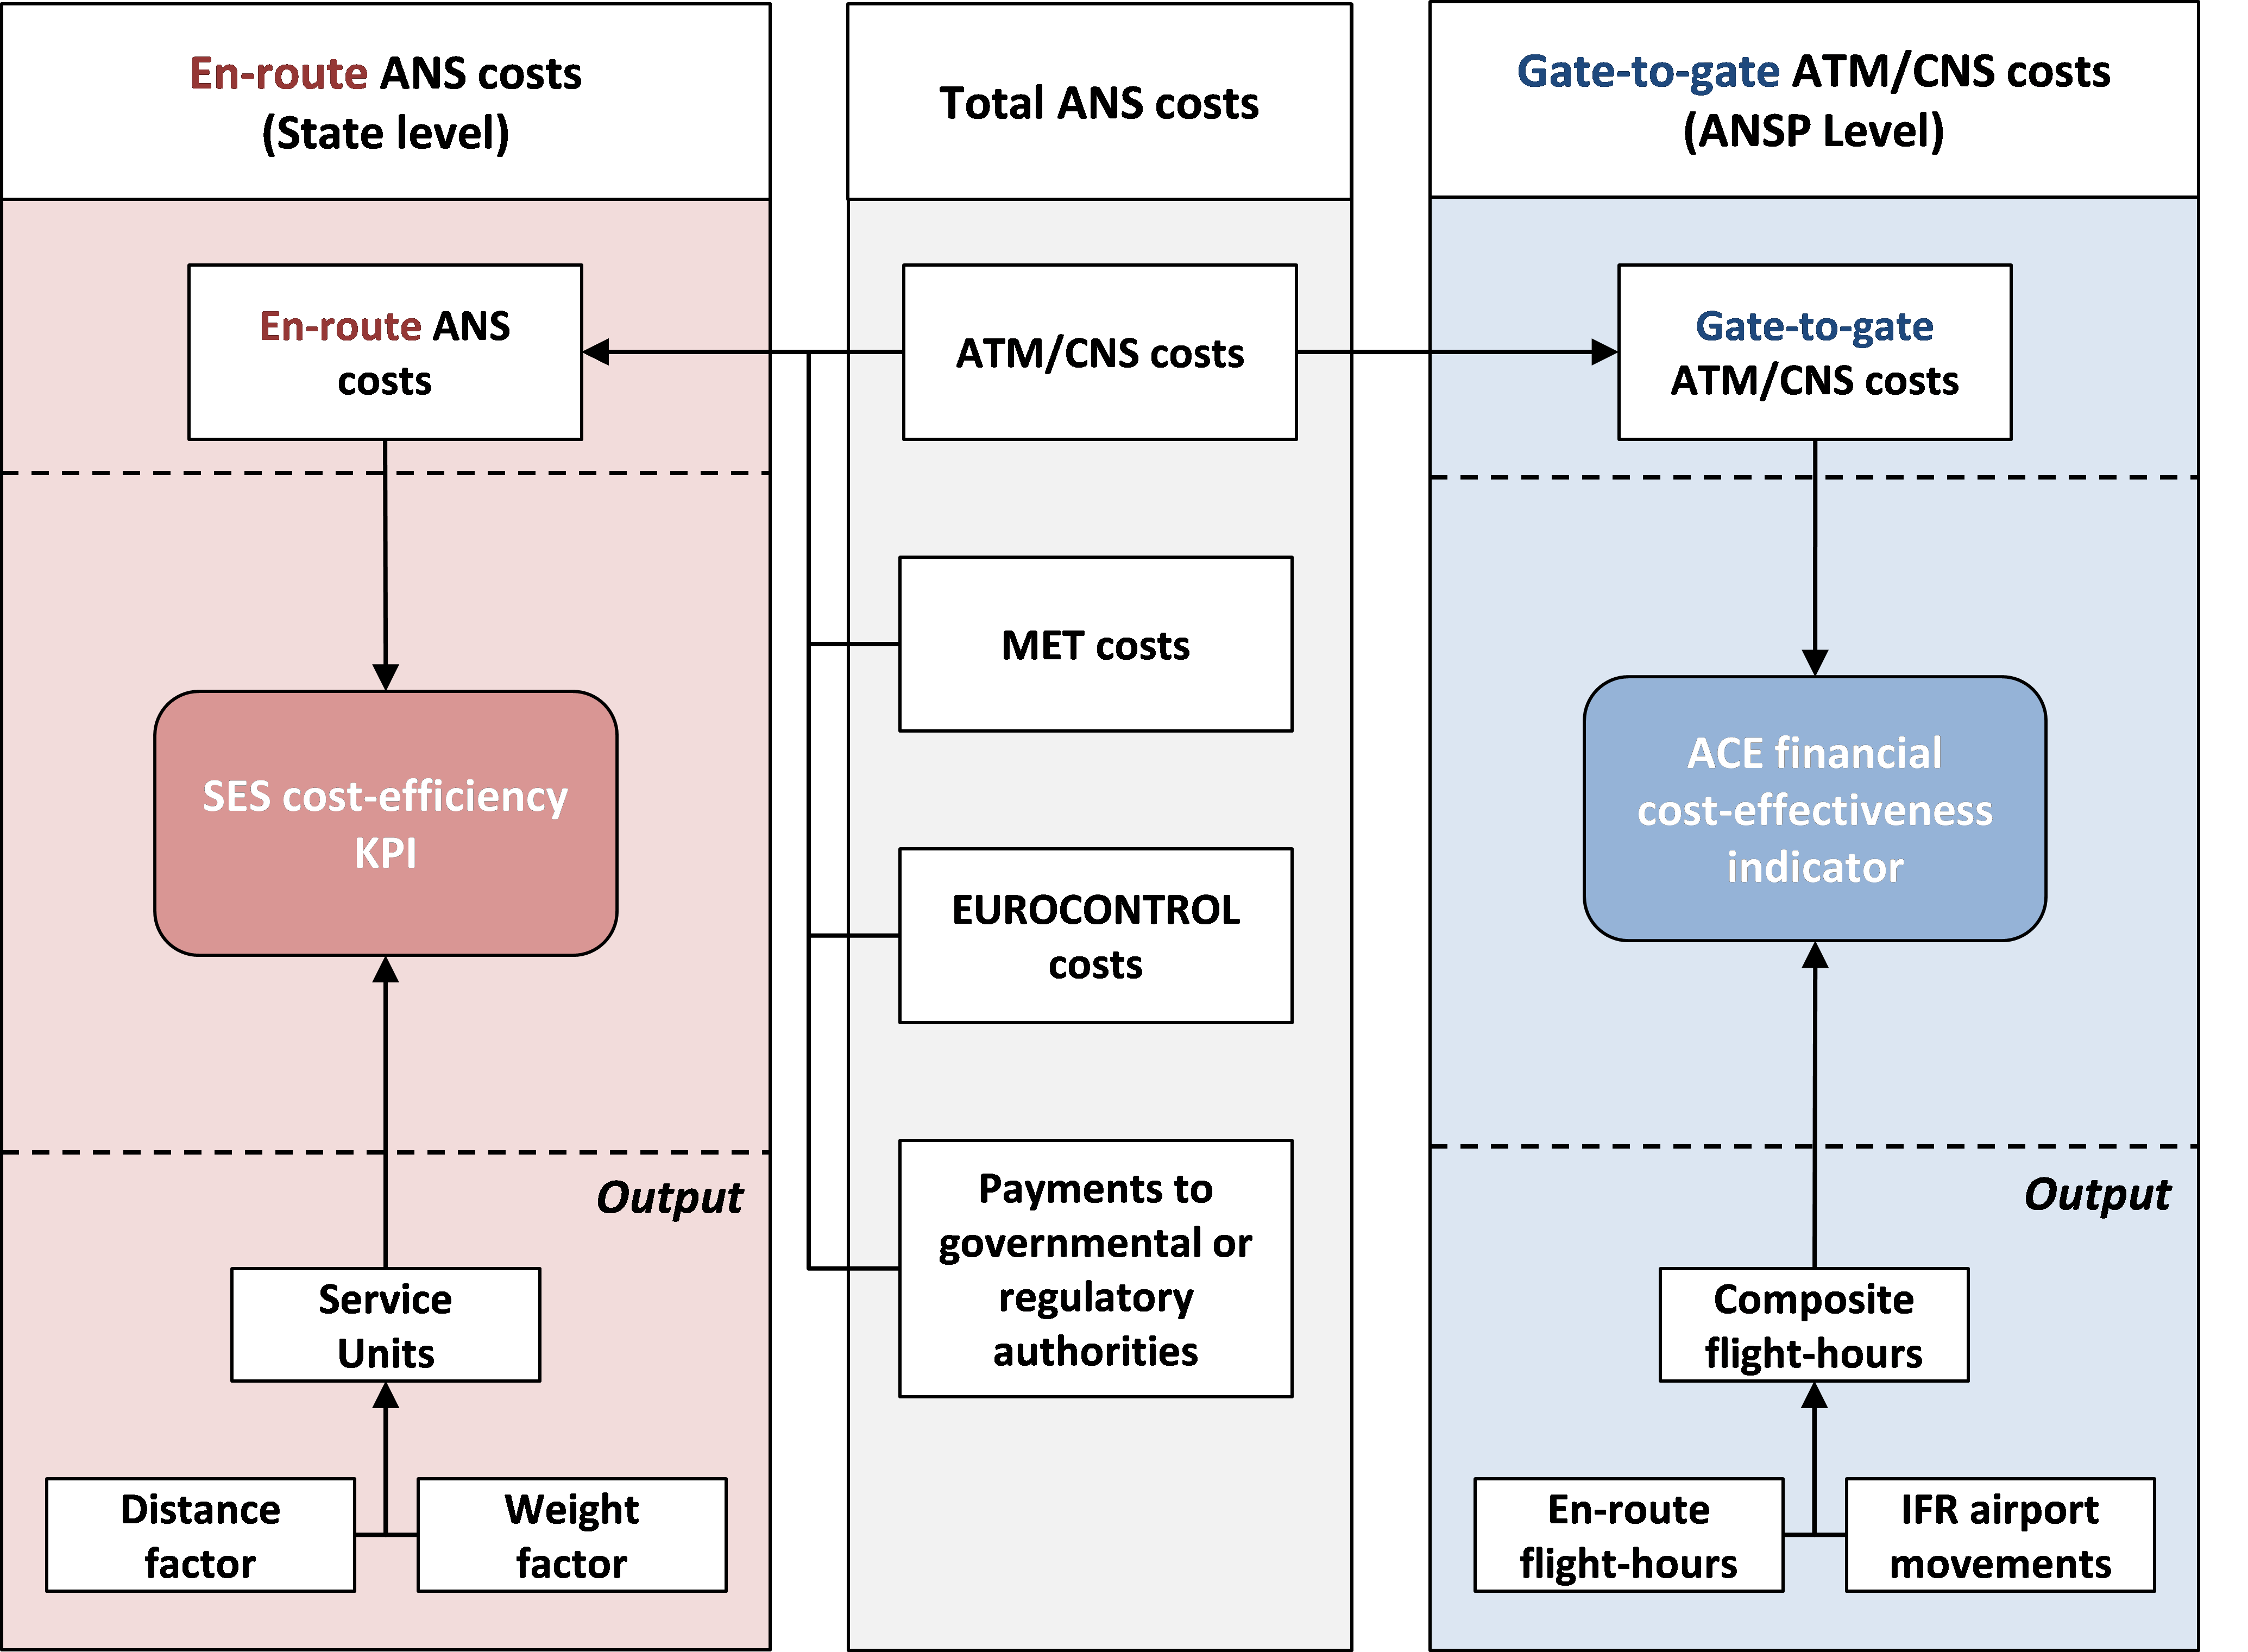
\includegraphics[width=0.9\linewidth,height=\textheight,keepaspectratio]{./images/image12.png}

}

\caption{\label{fig-indicator-and-kpi}ACE cost-effectiveness indicator
and SES cost-efficiency KPI}

\end{figure}%

As shown in Figure~\ref{fig-indicator-and-kpi}, the main differences
between the ACE financial cost-effectiveness indicator and the SES
en-route cost-efficiency KPI are the following:

\begin{itemize}
\item
  \textbf{Operational scope}: En-route and terminal costs are considered
  together when benchmarking the economic performance of ANSPs in the
  ACE analysis. It is important to consider a ``gate-to-gate''
  perspective because the boundaries used to allocate costs between
  en-route and terminal ANS vary between ANSPs and might introduce a
  bias in the cost-effectiveness analysis. On the other hand, the SES
  cost-efficiency KPI is computed for en-route and terminal ANS
  separately, for the purposes of the target-setting and/or monitoring
  processes.
\item
  \textbf{Service scope}: Total ANS costs (including costs relating to
  the ANSPs, METSPs, EUROCONTROL, and NSAs) are used to compute the SES
  cost-efficiency KPI, while only the ANSPs ATM/CNS provision costs are
  included in the ACE benchmarking analysis.
\item
  \textbf{Measure of the output}: The output metric used to compute the
  SES en-route cost-efficiency KPI is the number of en-route service
  units\footnote{\(\text{Service}\ \text{unit} = \text{distance factor} \times \ \sqrt{\frac{\text{MTOW}}{50}}\)
    According to EU Regulation 2019/317
    (\citeproc{ref-eu2019ux2f317}{European Commission 2019}, Annex VIII
    1.1 and 1.2), \emph{the en route service units shall be calculated
    as the product of the distance factor and the weight factor for the
    flight concerned. {[}\ldots{]} The distance factor in respect of a
    given charging zone shall be obtained by dividing by one hundred the
    number of kilometers flown.}}. This metric is a function of the
  aircraft weight and of the distance flown within a given charging
  zone. This is the metric which has been historically used to compute
  the en-route unit rate charged to airspace users. On the other hand,
  the ACE financial cost-effectiveness indicator is computed using
  composite flight-hours, which combine both flight-hours and IFR
  airport movements (see Section~\ref{sec-metric-and-framework}). It
  should be noted that the geographical area controlled by ANSPs
  operational units can substantially differ from the charging zones in
  case of delegation of ANS. The composite flight-hours therefore better
  reflect the operational activity performed by ANSPs, while service
  units are more appropriate when charging zones are considered.
\end{itemize}

\bookmarksetup{startatroot}

\chapter{Treatment of monetary factors in the ACE benchmarking
analysis}\label{treatment-of-monetary-factors-in-the-ace-benchmarking-analysis}

Presentation and comparison of historical series of financial data from
different countries poses problems, especially when different currencies
are involved, and inflation rates differ. There is a danger that
time-series comparisons can be distorted by transient variations in
exchange rates.

For this reason, the following approach has been adopted in the analysis
for allowing for inflation and exchange rate variation. The financial
elements of performance are assessed, for each year, in national
currency. They are then converted to national currency in year-N prices
using national inflation rates. Finally, for comparison purposes in
year-N, all national currencies are converted to Euros using the year-N
exchange rate.

This approach has the virtue that an ANSP's performance time series is
not distorted by transient changes in exchange rates over the period. It
does mean, however, that the performance figures for any ANSP in a given
year prior to year-N are not the same as the figures in that year's ACE
report, and cannot legitimately be compared with another ANSP's figures
for the same year. Cross-sectional comparison using the figures in the
ACE analytical report is only appropriate for year-N data.

The exchange rates used to convert the year-N data in Euros are those
provided by the ANSPs in their ACE data submission.

The historical inflation figures used in ACE are obtained from EUROSTAT
or from the International Monetary Fund when the information is not
available in EUROSTAT website. For the projections (future years), the
ANSPs' own assumptions concerning inflation rates are used.

Employment costs constitute a major part of ANS provision costs. Staff
has to be recruited in local labour markets, and therefore the
prevailing wage rates, for many different grades and types of staff,
will have a major influence on the overall employment costs. There are a
number of ways of measuring differences in prevailing wage levels
between different countries. In the ACE benchmarking reports, unit
employment costs are also compared when adjusted for Purchasing Power
Parities (PPPs). Purchasing Power Parities (PPPs) are currency
conversion rates that are applied to convert economic indicators in
national currency to an artificial common currency (Purchasing Power
Standard (PPS) for EUROSTAT statistics). The PPPs data used to adjust
most of the ANSPs employment costs is extracted from EUROSTAT.

For four countries (Armenia, Georgia, Moldova and Ukraine), PPP data is
not available in the EUROSTAT database. In these cases, the IMF database
is used. Since in the IMF database, the PPPs are expressed in local
currency per \textbf{international Dollar} rather than \textbf{PPS}, an
adjustment is made so that the figures used for ARMATS,
Sakaeronavigatsia, MOLDATSA and UkSATSE are as consistent as possible
with the data used for the rest of the ANSPs. The assumption underlying
this adjustment is that the difference in PPPs between two countries
shall be the same in the EUROSTAT and in the IMF databases.

There are some limitations\footnote{For instance, it is possible that,
  for a given country, the cost of living in regions where the ANSP
  headquarter and other main buildings (e.g.~ACCs) are located is higher
  than the average value computed at national level.} inherent to the
use of PPPs and for this reason the ACE data analysis does not put a
significant weight on results obtained with PPPs adjustments. PPPs are
nevertheless a useful analytical tool in the context of international
benchmarking.

\bookmarksetup{startatroot}

\chapter{Detailed information on the calculation of ACE
indicators}\label{detailed-information-on-the-calculation-of-ace-indicators}

\section{Cost-effectiveness
indicators}\label{cost-effectiveness-indicators}

The main indicators used in ACE to analyse ANSPs cost-effectiveness are:

\begin{itemize}
\item
  economic cost-effectiveness;
\item
  financial cost-effectiveness;
\item
  ATCO-hour productivity;
\item
  ATCO employment costs per ATCO-hour; and,
\item
  support costs per composite flight-hour.
\end{itemize}

The table below presents the formulas used to calculate these indicators
with reference to the
\href{https://www.eurocontrol.int/publication/eurocontrol-specification-economic-information-disclosure}{SEID}
item numbers.

\begin{longtable}[]{@{}
  >{\raggedright\arraybackslash}p{(\linewidth - 6\tabcolsep) * \real{0.0341}}
  >{\raggedright\arraybackslash}p{(\linewidth - 6\tabcolsep) * \real{0.1300}}
  >{\raggedright\arraybackslash}p{(\linewidth - 6\tabcolsep) * \real{0.2755}}
  >{\raggedright\arraybackslash}p{(\linewidth - 6\tabcolsep) * \real{0.5542}}@{}}
\toprule\noalign{}
\begin{minipage}[b]{\linewidth}\raggedright
\#
\end{minipage} & \begin{minipage}[b]{\linewidth}\raggedright
Indicator
\end{minipage} & \begin{minipage}[b]{\linewidth}\raggedright
Formula
\end{minipage} & \begin{minipage}[b]{\linewidth}\raggedright
Source
\end{minipage} \\
\midrule\noalign{}
\endhead
\bottomrule\noalign{}
\endlastfoot
1 & Composite flight-hours & En-route flight-hours +(0.27×IFR airport
movements) & \textbf{\emph{En-route flight-hours:}} Item D16,
continental ANS

\textbf{\emph{IFR airport movements:}} Item D18, SES airports + Non-SES
airports

\textbf{0.27} is the two-digits rounded weighting factor (see
Chapter~\ref{sec-method}) \\
2 & Economic cost-effectiveness & (Total service provision costs+Total
costs of ATFM delays)/(Composite flight-hours) & \textbf{\emph{Total
service provision costs:}} Item A15 (en-route + terminal columns)

\textbf{\emph{Total costs of ATFM delays:}} Minutes of ATFM delays
extracted from the Network manager database, monetarised using the cost
of a minute of ATFM delays (see Chapter~\ref{sec-delay-cef})

\textbf{\emph{Composite flight-hours:}} Formula \#1 \\
3 & Financial cost-effectiveness & (Total service provision
costs)/(Composite flight-hours) & \textbf{\emph{Total service provision
costs:}} Item A15 (en-route + terminal columns)

\textbf{\emph{Composite flight-hours:}} Formula \#1 \\
4 & ATCO-hour productivity & (Composite flight-hour)/(Sum of ATCO in OPS
hours on duty) & \textbf{\emph{Composite flight-hours:}} Formula \#1

\textbf{\emph{Sum of ATCO in OPS hours on duty:}} Item D22 (ACCs +
APPs+TWRs columns) \\
5 & ATCO employment costs per ATCO-hour & (Staff costs for ATCOs in
OPS)/(Sum of ATCO in OPS hours on duty) & \textbf{\emph{Staff costs for
ATCOs in OPS:}} Item C23 (en-route + terminal columns)

\textbf{\emph{Sum of ATCO in OPS hours on duty:}} Item D22 (ACCs +
APPs+TWRs columns) \\
6 & Support costs per composite flight-hour & (Total service provision
costs-ATCOs in OPS Employment costs)/(Composite flight-hours) &
\textbf{\emph{Total service provision costs:}} Item A15 (en-route +
terminal columns)

\textbf{\emph{ATCOs in OPS Employment costs:}} Item C23 (en-route +
terminal columns)

\textbf{\emph{Composite flight-hours:}} Formula \#1 \\
\end{longtable}

\section{Financial indicators used to monitor ANSPs liquidity and cash
situation}\label{financial-indicators-used-to-monitor-ansps-liquidity-and-cash-situation}

The current ratio and cash-on-hand days indicators are used in ACE
report to analyse ANSPs financial situation. The formulas and sources of
data used for calculation are presented in the table below.

\begin{longtable}[]{@{}
  >{\raggedright\arraybackslash}p{(\linewidth - 6\tabcolsep) * \real{0.0710}}
  >{\raggedright\arraybackslash}p{(\linewidth - 6\tabcolsep) * \real{0.1183}}
  >{\raggedright\arraybackslash}p{(\linewidth - 6\tabcolsep) * \real{0.4260}}
  >{\raggedright\arraybackslash}p{(\linewidth - 6\tabcolsep) * \real{0.3728}}@{}}
\toprule\noalign{}
\begin{minipage}[b]{\linewidth}\raggedright
\#
\end{minipage} & \begin{minipage}[b]{\linewidth}\raggedright
Indicator
\end{minipage} & \begin{minipage}[b]{\linewidth}\raggedright
Formula
\end{minipage} & \begin{minipage}[b]{\linewidth}\raggedright
Source
\end{minipage} \\
\midrule\noalign{}
\endhead
\bottomrule\noalign{}
\endlastfoot
1 & Current ratio & (Current assets)/(Current liabilities) &
\textbf{\emph{Current assets:}} Item B15 (total ANS column)

\textbf{\emph{Current liabilities:}} Item B30, (total ANS column) \\
2 & Cash-on-hand days & (Cash in hand or at bank)/(Staff costs+Non-staff
operating costs)×365 & \textbf{\emph{Cash in hand or at bank}}: Item B18
(total ANS column)

\textbf{\emph{Staff costs:}} Item A16, (total ANS column)

\textbf{\emph{Non-staff operating costs:}} Item A17 (total ANS
column) \\
\end{longtable}

\bookmarksetup{startatroot}

\chapter*{References}\label{references}
\addcontentsline{toc}{chapter}{References}

\markboth{References}{References}

\phantomsection\label{refs}
\begin{CSLReferences}{1}{0}
\bibitem[\citeproctext]{ref-seid}
EUROCONTROL. 2012. {``Specification for {Economic Information
Disclosure}.''} Specification EUROCONTROL-SPEC-117, ver 3.0. {Brussels,
Belgium}: {EUROCONTROL}.
\url{https://www.eurocontrol.int/ACE/Supporting-Documents/SEID3.0.pdf}.

\bibitem[\citeproctext]{ref-eu2019ux2f317}
European Commission. 2019. {``Commission {Implementing Regulation}
({EU}) 2019/317 of 11 {February} 2019 Laying down a Performance and
Charging Scheme in the Single {European} Sky and Repealing {Implementing
Regulations} ({EU}) {No} 390/2013 and ({EU}) {No} 391/2013 ({Text} with
{EEA} Relevance.).''} {Official Journal of the European Union}.
\url{https://eur-lex.europa.eu/eli/reg_impl/2019/317/oj}.

\bibitem[\citeproctext]{ref-ec550ux2f2004}
European Parliament, and Council of the European Union. 2004.
{``Regulation ({EC}) {No} 550/2004 of the {European Parliament} and of
the {Council} of 10 {March} 2004 on the Provision of Air Navigation
Services in the Single {European} Sky (the Service Provision
{Regulation}) ({Text} with {EEA} Relevance).''} {Official Journal of the
European Union}. \url{https://eur-lex.europa.eu/eli/reg/2004/550/oj}.

\bibitem[\citeproctext]{ref-prc01ux2f2005}
Performance Review Commission. 2005. {``Total {Factor Productivity} of
{European Air Navigation Services Providers}: {Basic Concepts} and
{Empirical Application}.''} \{\{PRU Technical Note\}\} 01/2005.
{Brussels, Belgium}: {EUROCONTROL}.
\url{https://www.eurocontrol.int/publication/total-factor-productivity-european-air-navigation-services-providers}.

\bibitem[\citeproctext]{ref-ace_reports}
Performance Review Unit. 2023. {``{ATM Cost-Effectiveness} ({ACE})
{Benchmarking Reports}.''}
\url{https://ansperformance.eu/publications/prc/ace/}.

\bibitem[\citeproctext]{ref-pc88}
Permanent Commission for the Safety of Air Navigation. 2015. {``Decision
{No}. 88 of the {EUROCONTROL Permanent Commission}.''} {Brussels,
Belgium}: {EUROCONTROL}.
\url{https://www.eurocontrol.int/sites/default/files/content/documents/official-documents/pc/commission-act/ecn-decisions-88en.pdf}.

\bibitem[\citeproctext]{ref-uow:costofdelay}
University of Westminster. 2015. {``European Airline Delay Cost
Reference Values.''}
\url{https://www.eurocontrol.int/publication/european-airline-delay-cost-reference-values}.

\end{CSLReferences}

\bookmarksetup{startatroot}

\chapter*{Disclaimer}\label{disclaimer}
\addcontentsline{toc}{chapter}{Disclaimer}

\markboth{Disclaimer}{Disclaimer}

The Performance Review Unit (PRU) has made every effort to ensure that
the information and analysis contained in this document are as accurate
and complete as possible.

Should you find any errors or inconsistencies we would be grateful if
you could please bring them to the PRU's attention.

The PRU's e-mail address is
\href{mailto:PRU-Support@eurocontrol.int?subject=Feedback:\%20ACE\%20Handbook}{pru-support@eurocontrol.int}


\backmatter


\end{document}
